\documentclass[11pt, oneside]{book}
\usepackage{setspace}
\newcommand{\HRule}{\rule{\linewidth}{0.5mm}}
%\usepackage{fancyhdr}
\usepackage[T1]{fontenc}
\usepackage[margin=1.1in]{geometry}
\usepackage[utf8]{inputenc}
\usepackage{epsfig}
%\usepackage{subfigure}
\usepackage{calc}
\usepackage{dsfont}
\usepackage{amssymb}
\usepackage{amstext}
\usepackage{amsmath}
\usepackage{amsthm}
\usepackage{mathtools}
\usepackage{amsfonts}
\usepackage{multicol}
\usepackage{mathtools,xparse}
\usepackage[hidelinks]{hyperref}
\usepackage{booktabs}
\usepackage{enumitem}
\usepackage{calligra}
\usepackage{float}
\usepackage{wrapfig}

\usepackage[table] {xcolor}
\usepackage{lipsum}
\usepackage{caption}
\usepackage{subcaption}
\usepackage{graphicx}
\usepackage{todonotes}
 % % % REFERENCES
%
\usepackage[numbers]{natbib}
\usepackage{amsmath}
%
% % % %

% % % %
%
\usepackage[labelfont=bf]{caption} %labelfont is to make the Figure X.X: in bold
\usepackage[titletoc,toc,page]{appendix}
%
% % % %

% % % % TableFootnote
%
\newcommand*{\savedfootnotes}{}
\newcommand*{\resetsavedfootnotes}{\global\let\savedfootnotes\empty}
\newcommand{\tablefootnote}[1]
{
	\footnotemark
	\xdef\savedfootnotes
	{\unexpanded\expandafter{\savedfootnotes}\noexpand\footnotetext{#1}}
}
\edef\endtable
{
	\aftergroup\noexpand\savedfootnotes
	\aftergroup\noexpand\resetsavedfootnotes
	\unexpanded\expandafter{\endtable}
}
%
% % % %

% % % % Norms
%
\DeclarePairedDelimiter{\abs}{\lvert}{\rvert}
\DeclarePairedDelimiter{\norm}{\lVert}{\rVert}
\NewDocumentCommand{\normL}{ s O{} m }{
	\IfBooleanTF{#1}{\norm*{#3}}{\norm[#2]{#3}}_{L_2(\Omega)}%
}
%
% % % %

\setcounter{secnumdepth}{3}
\setcounter{tocdepth}{3}

\newcommand\phantomarrow[2]{
	\setbox0=\hbox{$\displaystyle #1\to$}
	\hbox to \wd0{
		$#2\mapstochar
		\cleaders\hbox{$\mkern-1mu\relbar\mkern-3mu$}\hfill
		\mkern-7mu\rightarrow$}
	\,}

\graphicspath{{Images//},{sections//},{Images/qualitative_tests/}}
\input epsf

%\subfigtopskip=0pt
%\subfigcapskip=0pt
%\subfigbottomskip=0pt


% % % Sections 
\usepackage{titlesec}
\titleformat{\chapter}[hang]{\Huge\bfseries}{\thechapter}{15pt}{\Huge\bfseries}
%\titlespacing{\chapter}{0pt}{-50pt}{20pt}


%Bigger elements in matrix
\makeatletter
\renewcommand*\env@matrix[1][\arraystretch]{%
	\edef\arraystretch{#1}%
	\hskip -\arraycolsep
	\let\@ifnextchar\new@ifnextchar
	\array{*\c@MaxMatrixCols c}}
\makeatother

% % DEFINITIONS, propositions enviornment
\newtheorem{definition}{Definition}
\newtheorem{proposition}{Proposition}
% % 


% ALGORITHMS
\usepackage{algorithm}
\usepackage{algorithmicx}
%\usepackage{algorithmic}
\usepackage{algpseudocode}
%\usepackage[noend]{algpseudocode}
\usepackage{pifont}
%\algdisablelines
\usepackage{xpatch}

% ACRONYMS AND GLOSSARIES
\usepackage[acronym]{glossaries}
\makeglossaries
\newacronym{lfs}{LFS}{Labour Force Survey}
\newacronym{gcd}{GCD}{Greatest Common Divisor}
\newacronym{lcm}{LCM}{Least Common Multiple}
% ACRONYMS AND GLOSSARIES

\makeatletter
\xpatchcmd{\algorithmic}{\itemsep\z@}{\itemsep=2ex plus2pt}{}{}
\def\BState{\State\hskip-\ALG@thistlm}
\makeatother

%\setlength{\arrayrulewidth}{1mm}
%\setlength{\tabcolsep}{18pt}
%\renewcommand{\arraystretch}{1.5}

\newcommand{\old}{\texttt{algorithmic}}
\newcommand{\euk}{Euclid}
\newcommand\ASTART{\bigskip\noindent\begin{minipage}[b]{0.5\linewidth}}
	\newcommand\ACONTINUE{\end{minipage}\begin{minipage}[b]{0.5\linewidth}}
	\newcommand\AENDSKIP{\end{minipage}\bigskip}
\newcommand\AEND{\end{minipage}}
%\renewcommand{\algorithmicrequire}{\textbf{Input:}}
%\renewcommand{\algorithmicensure}{\textbf{Output:}}
\newcommand{\algorithmicbreak}{\textbf{break}}

\algdef{SE}[DOWHILE]{Do}{doWhile}{\algorithmicdo}[1]{\algorithmicwhile\ #1}%

% % % % % % % % % % % % % % % % % % % %

\begin{document}

%\title{Cage active contours: Extension to color spaces and
%		 application to image morphing }
%
%\keywords{The paper must have at least one keyword. The text must be set to 9-point font size and without the use of bold or italic font style. For more than one keyword, please use a comma as a separator. Keywords must be titlecased.}
%
%
%\onecolumn \maketitle \normalsize \vfill
\setcounter{page}{3}
%\pagestyle{fancy}
\begin{titlepage}
	
	\begin{figure}[t]
		\centering
		
\includegraphics[scale=0.4]{images/upc_ub_urv}
	\end{figure}    
	
	
	\begin{center}
		
		{\large \uppercase{Universitat politècnica de Catalunya}} \medskip \\
		{\large \uppercase{Universitat de Barcelona}} \medskip \\
		{\large \uppercase{Universitat Rovira i Virgili}} \medskip \\
		\vspace*{1cm}
		\begin{center}
			\Large	\bf   Master in Artificial Intelligence
		\end{center}
		

		{\Large Master of Science Thesis} \vspace*{1.0cm} \\
		\HRule \\[0.4cm]
		{ \huge \bfseries Synthetic Data Generation for Deep Learning in Small Datasets }\\[0.4cm] % Title of your document

		\HRule \\[1.cm]
	\end{center}

	
	\thispagestyle{empty}
	\begin{center}
	\Large	\bf Hadi Keivan Ekbatani\\
	\end{center}
	\begin{center}
		{\large \uppercase{Facultat d'informàtica de Barcelona (FIB)}} \medskip \\
		{\large \uppercase{Facultat de Matemàtiques (UB)}} \medskip \\
		{\large \uppercase{Escola tècnica superior d'enginyeria (URV)}} \medskip \\
	\end{center}
	\vspace*{1. cm}
	\begin{center} 
		\begin{multicols}{2}	
		{\large Supervisor:}
		
		
		\medskip %\medskip\smallskip
		
		{\Large\bf Oriol Pujol Vila}
		
		\medskip %\medskip
		
		{Department of analysis\\
			and applied Mathematics,\\
			 Universitat de Barcelona (UB)}
		
		\medskip
		
		{\large Co-supervisor:}
		
		\medskip
				
		{\Large\bf Santiago Segui Mesquida}
			
		\medskip %\medskip

		{Department of analysis\\
			and applied Mathematics,\\
			Universitat de Barcelona (UB)}
		\end{multicols}
		\medskip\medskip\medskip\medskip\medskip
		
		% This has obviously to be changed
		%\vspace*{1\baselineskip}
		\today
		
	\end{center}

\end{titlepage}
\thispagestyle{empty}

\thispagestyle{empty}
\chapter*{Acknowledgments}
\thispagestyle{empty}

I would like to sincerely thank my supervisors Oriol Pujol and Santi Segui for their support, guidance and mentorship. I greatly appreciate their demanding and inquisitive scientific attitude, while keeping always a calm and positive mindset. They are, in my mind, an inspiring example of what university professors should be.

Furthermore, I would also like to dedicate this master thesis to my beloved parents and sister for their unsparing supports. My gratitude knows no bounds.

Another special acknowledgment must be made to my friends in the master: Denis, Jeroni, Philipp, Pablo, Lorenzo, Iosu, Ferran and many others for the endless studying hours, morning coffees after crunching the brutal assignments all night long, valuable and constructive discussions which allowed me carry out this program. 
 



\pagenumbering{arabic}
\setcounter{page}{0}
\clearpage

%Table of contents
\newpage
\pagenumbering{roman} % Roman numerals
\chapter*{Abstract}
\thispagestyle{empty}

This master's thesis provides an analysis on the generation of synthetic datasets as a pertinent substitute for missing large training sets in learning algorithms. Furthermore, it endeavors to enhance feature detection in learning to count problems by application of Deep Learning (DL) algorithms. 

%This master's thesis endeavors to enhance feature detection in learning to count problems by application of deep learning algorithms. Furthermore, it proposes a new way to reduce data annotation efforts through incorporation of synthetically created datasets in the learning process. 

In the course of our research, we introduce two highly realistic synthetically created sets of images to train proposed Deep Convolutional Neural Networks (DCNN) to approach two tasks: learning to count even-digits and counting the number of pedestrians in a walkway. In the former case, we analyze the applicability of deep features as a surrogate to hand-crafted features for understanding the underlying representations. Subsequently, in the latter task, the features learned by training the DCNN on synthetic images, are tested on a small real-world dataset of pedestrians to overcome the inefficiency of deep learning algorithms when facing lack of data.

%In the course of our research, we propose convolutional deep neural networks to approach two tasks: learning to count even-digits and counting the number of pedestrians in a walkway, along with the supporting synthetically created datasets. In the former case, we analyze the applicability of deep features as a surrogate to hand-crafted features for understanding the underlying representations. Subsequently, in the latter task, the features learned by training the deep CNN on synthetic images, are tested on a small real-world dataset of pedestrians to overcome the inefficiency of deep learning algorithms when facing lack of data.

To evaluate our methodology, we present an empirical experiment followed by comparison to the state-of-the-art methods. Improving the cutting-edge solutions, our results demonstrate the suitability of deep models to learn objects features for counting tasks in Computer Vision (CV). Furthermore, obtaining notable results on real-word problems compared to previous highly specialized approaches, suggests synthetic data as a viable workaround for application of deep learning to problems with small datasets. 

 



     



 


\tableofcontents

\listoffigures

\listoftables



\newpage
\pagenumbering{arabic} % Normal numerals

\newpage\null\thispagestyle{empty}\newpage
\part{title}\chapter{Introduction}
\label{sec:introduction}
\section{Motivations}
%2. What is the background, the context, in which the research took place? 
The concept of learning to count is an important educational/developmental milestone  which constitutes the most fundamental idea of mathematics. In Computer Vision\cite{umbaugh1997computer}, the counting problem is the estimation of number of objects in a still image or video frame. Learning to count visual objects is a new approach towards dealing with detecting object in the images and video, which has been recently proffered in the literature\cite{viola2005detecting, rabaud2006counting, kong2005counting, chan2008privacy, segui2015learning}. It arises in many real-world applications, including cell counting in microscopic images\cite{flaccavento2011learning}, monitoring crowds in surveillance systems\cite{rahmalan2006crowd, valera2005intelligent}, and performing wildlife census or counting the number of trees in an aerial image of a forest\cite{brandtberg1998automated, pollock1996automatic}\cite{NIPS2010_4043}. 

Artificial intelligence and computer vision share topics such as pattern recognition and machine learning\cite{michalski2013machine, mitchell1997machine} techniques. Consequently, computer vision is sometimes seen as a part of the artificial intelligence field or the computer science field in general. Recent machine learning methods applied for computer vision tasks, require large number of data for the learning process. To learn to count the object of interest in an image or video, various object features need to be designed, extracted or detected during the learning phase. The complexity of feature detection process in vision tasks, restrict their usage in large-scale computer vision applications thus demanding more efficient solutions to alleviate, expedite and improve this process. 

\indent One recent and commonly used method to facilitate feature detection process is application of deep Convolutional Neural Networks(CNN)\cite{szegedy2015going, krizhevsky2012imagenet, lecun1995convolutional, sermanet2013overfeat, ji20133d, taylor2010convolutional}. One of the promises of deep CNN is replacing handcrafted features with efficient algorithms for unsupervised or semi-supervised feature learning and hierarchical feature extraction\cite{song2013hierarchical}. CNNs have been claimed and practically proven to achieve the most assuring performance in different vision benchmark problems concerning feature detection and classification\cite{ciresan2011flexible, szegedy2015going, ciresan2012multi}. 

\section{Objectives}
This work sets forward several objectives:
\begin{enumerate}
	\item To apply deep CNN for feature detection and classification in a learning to count problem where the concept of interest will be counted by no giving explicit information about what we are counting to the system, except for its multiplicity in the image. 
	\item To synthetically create datasets of images, as realistic as possible, and completely automatically annotated for CNN to train with.
	\item To explore the behavior of proposed algorithm on synthetic datasets of different types comparing the performance with a state-of-the-art outcomes\cite{segui2015learning}.   
	\item To analyze the performance of designed system on real world crowd counting problem comparing the results with state-of-the-art results\cite{chan2008privacy}.   

\end{enumerate}
\section{Contributions}
This thesis contains the following contributions:
\begin{enumerate}
	\item It proposes the problem of object representation as an indirect learning problem casted as learning to count strategy. The devised algorithm is capable of counting the number of pedestrians in the image that does not depend on object detection or feature tracking. The model is also privacy-preserving in a sense that it can be implemented with hardware that does not produce a visual record of the individuals in the scene. 
	\item It provides a synthetically generated and automatically labeled dataset of pedestrians using unlabeled University of California San Diego(UCSD) pedestrian dataset used in \cite{mahadevan2010anomaly}, to train a counting deep convolutional neural network which is adequate for apprehending the underlying representations of the learned features. To this end, we describe a counting problem for MNIST dataset to demonstrate the capability of the internal representation of the network for classifying digits with no direct supervising while training. 
	\item The proposed model is able to count the number of people in the real and unseen dataset using the features learned by training the network on synthetic training set. To our knowledge, this is the first crowd counting system trained by synthetic data that successfully operates continuously on real data. 
	\item Along with the validation of our proposal in the following ways:
	\begin{itemize}
		\item First, we learn to count even hand-written digits using MNIST dataset. 
		\item Second, we validate the system quantitatively on a large synthetic dataset of pedestrian, containing 100,000 images with maximum 30 pedestrians in each image. 
		\item Last but not least, we count the number of pedestrians in the manually labeled dataset of 3375 images provided by[\citeauthor*{chan2013ground}, \citeyear{chan2013ground}]. 
	\end{itemize}
	
\end{enumerate}

\section{Organization}

This report takes off with the review of Deep Learning(DL) as a branch of Artificial Intelligence (AI) which deep convolutional neural networks belong to, and moves on to introduce a deep CNN's basic architecture and components in details along with the definition of applied optimization methods and hyper-parameters in our work (Section 2.1). This section ends with a review of state of the art (Section 2.2). 

In section 4, we describe our proposal for constructing a deep neural network to tackle feature detection issue learning to count problems. 

Section 5 revolves around the empirical experiments and analysis along with the peculiarities of proposed data creation process and network modeling.  

Lastly, in Chapter 6 we conclude the report with a short summary of the scope of work conducted and the new areas of research that this master thesis has opened.

\chapter{Background and Definitions}
\label{sec:Background}
% neural networks 
In this section, we go over the preliminarily concepts that help understand the contributions of this work. We start by looking at the family of methods to which deep convolutional neural networks belong, followed by a more detailed look at DCNNs in question by describing the main components of the method.

\section{Deep Learning}
\label{sec:dl}
%Today, \textit{Artificial Intelligence(AI)} is a thriving field with many practical applications and active research topics. We look to intelligent software to automate routine labor, understand speech or images, make diagnoses in medicine and support basic scientific research. 
One of the central challenges of artificial intelligence is solving the tasks that are easy for people to perform but hard for them to describe formally -- problems that we solve intuitively, that feel automatic, like recognizing spoken words or faces in images. One approach to that challenge is to allow computers to learn from experience and understand the world in terms of a hierarchy of concepts, where each concept is defined in terms of its relation to simpler concepts. This hierarchy of concepts allows the computer to learn complex notions by building them out of simpler ones. If we draw a graph showing how these concepts are built on top of each other, it would be a deep graph with many layers. For this reason, we call this approach \textit{Deep Learning} \cite{Goodfellow-et-al-2016-Book}.

Modern deep learning provides a very powerful framework specially for supervised learning. By adding more layers and more units within a layer, a deep network can represent functions of increasing complexity. Most tasks that consist of mapping an input vector to an output vector, and that are easy for a human-being to perform quickly, can be accomplished via deep learning, given sufficiently large models and datasets of labeled training examples. Other tasks that cannot be described as associating one vector to another, or that are difficult enough such that a person would require time to think and reflect in order to accomplish the task, remain beyond the scope of deep learning for now \cite{Goodfellow-et-al-2016-Book}.

In other words,  deep learning is a new area of Machine Learning (ML) research, which has been introduced with the objective of moving ML closer to one of its original goals: artificial intelligence. DL is about learning multiple levels of representation and abstraction that help to make sense of data such as images, sound and text.  

Various deep learning architectures involve Artificial Neural Networks (ANN). Networks such as \textit{deep neural networks}, \textit{deep convolutional neural networks},\textit{ deep belief networks} and \textit{recurrent neural networks} have been applied to fields like computer vision, automatic speech recognition or natural language processing where they have set the state-of-the-art in recent years, as reviewed by \citeauthor{bengio2009learning} in \cite{bengio2009learning, bengio2013deep}. 

Besides improving the accuracy on different pattern recognition problems, one of the fundamental goals of DL is to move machine learning towards the automatic discovery of multiple levels of representation, reducing the need for feature extractors developed by domain experts~\cite{bengio2013deep}. This is especially important, as noted by \citeauthor{bengio2009learning} in \cite{bengio2009learning}, for domains where the features are hard to formalize, such as for object recognition and detection tasks.

In the task of object detection, deep architectures have been widely used to achieve state-of-the-art results, as in \cite{krizhevsky2012imagenet}, where the top published results use Convolutional Neural Networks (CNN) \cite{ciresan2012multi}. Among all deep learning techniques, we will apply deep convolutional neural networks to tackle a specific vision problem. However, prior to delving into deep CNN, we intend to allude to the basic concept of neural networks and deep NN briefly, in order to help understand the proposed method in this Master thesis.

\section{Artificial Neural Networks}

Artificial Neural Networks (ANN) are mathematical models that use a collection of simple computational units, called Neurons, interlinked in a network. These models are used in a variety of pattern recognition tasks, such as speech recognition, object detection, identification of cancerous cells, among others \cite{hertz1991introduction}. ANNs date back to 1943, with work by McCulloch \cite{mcculloch1943logical}. The motivation for studying neural networks was the fact that the human brain was superior to a computer at many tasks, a statement that holds true even today for tasks such as recognizing objects and faces, in spite of the huge advances in the processing speed in modern computers.

The neuron is the basic unit on Artificial Neural Networks, and it is used to construct more powerful models. A typical set of equations to describe Neural Networks is provided in \cite{williams1986learning}, and is also listed below for completeness. A single neuron implements a mathematical function given its inputs, to provide an output, as described in equation ~\ref{eq:neuron} and illustrated in figure~\ref{fig:neuron}.

\begin{figure}[H]
	\centering
	{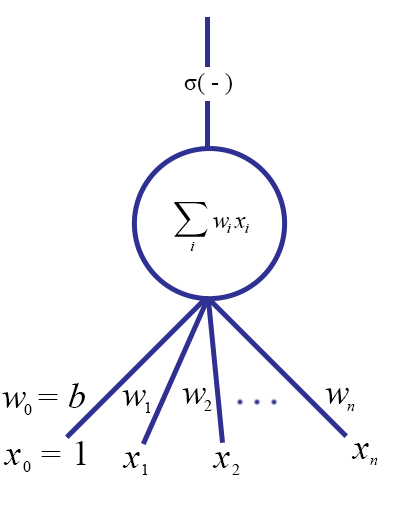
\includegraphics[width=0.34\textwidth]{images/neuron2}}
	\caption{A single artificial neuron}
	\label{fig:neuron}
\end{figure}

\begin{equation}
f(x) = \sigma(\sum\limits_{i=1}^{n}x_iw_i + b) 
\label{eq:neuron}
\end{equation}

In this equation, $x_i$ is the input \textit{i}, $w_i$ is the weight associated with input \textit{i}, \textit{b} is a bias term and $\sigma$ is a non-linear function. Common non-linear functions are \textit{Rectified Linear Unit} non-linearity, and\textit{ Sigmoid} function.

\subsection{Activation Functions}
\label{sec:actfun}
To go from one layer to the next in a NN, units compute a weighted sum of their inputs from the previous layer and pass the result through a non-linear activation function \cite{lecun2015deep}. There are many possible choices for the non-linear activation functions in a multi-layered network, and the choice of activation functions for the hidden units may often be different from that for the output units. This is a consequence of the fact the hidden and output units perform different roles \cite{bishop1995neural}. 

\indent At present, the most popular non-linear function is the Rectified Linear Units (ReLU), which is simply the half-wave rectifier $f(z) = max(z, 0)$. In the past decades, neural nets used smoother non-linearities, such as $tanh(z)$ or $1/(1+ exp(-z))$, but ReLU typically learns much faster in networks with many layers, allowing training of a deep supervised network without unsupervised pre-training \cite{lecun2015deep}. A rectified linear unit has been illustrated in figure~\ref{fig:relu}

\begin{figure}[H]
	\centering
	{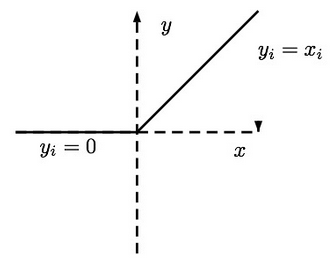
\includegraphics[width=0.4\textwidth]{images/relu}}
	\caption{A Rectified Linear Unit (ReLU)}
	\label{fig:relu}
\end{figure}

\indent The rectifier activation function allows a network to easily obtain sparse representations. For example, after uniform initialization of the weights, around 50\% of hidden units continuous output values are real zeros, and this fraction can easily increase with sparsity-including regularization. Apart from being more biologically plausible, sparsity also leads to mathematical advantages. On the other hand, one may hypothesize that the hard saturation at 0 may hurt optimization by blocking gradient back-propagation. However, experimental results done by \citeauthor{glorot2011deep} suggest that hard zeros can actually help in  supervised training \cite{glorot2011deep}.  


\subsection{Multi-layer Neural Network}

Models based on a single neuron, also called Perceptron, have severe limitations. As noted by \citeauthor{preparata2012computational} in \cite{preparata2012computational}, a perceptron cannot model data that is not linearly separable, such as modeling a simple XOR operator. On the other hand, as shown by \citet{hornik1989multilayer}, Multi-layer Neural Networks are universal approximators, that is: they can approximate any measurable function to any desired degree of accuracy.


A neural network of three or above layers of neurons shapes a \textit{Multi-layer Neural network} where the first layer is composed of the inputs to the neural network, it is followed by one or more \textit{hidden} layers, up to a last layer that contains the outputs of the network. In the simplest configuration, each layer \textit{l} is fully connected with the adjacent layers $(l - 1 ,~ l + 1)$, and produces an output vector $y^{l}$ given the output vector of the previous layer y $^{l-1}$. The output of a layer is calculated by applying the neuron activation function for all neurons on the layer, as noted in equation ~\ref{eq:multi}, where $W^{l}$ is a matrix of weights assigned to each pair of neurons from layer \textit{l} and $l - 1$, and $b^{l}$ is a vector of bias terms for each neuron in layer \textit{l}.

\begin{equation}
y^{l} = \sigma(W^{l}y^{l-1}+ b^{l}) 
\label{eq:multi}
\end{equation}


\begin{figure}[H]
	\centering
	{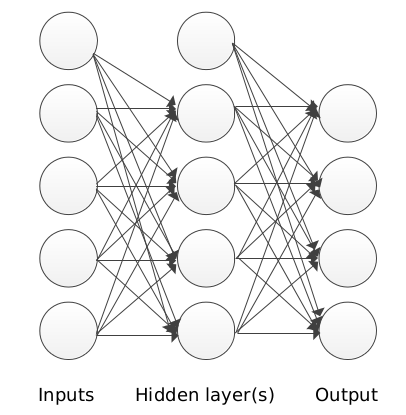
\includegraphics[width=0.45\textwidth]{images/mann}}
	\caption{A neural network composed of three layers}
	\label{fig:multi}
\end{figure}

\subsubsection{Training Objective} 
In order to train the model, an error function, also called \textit{loss function}, is defined. This function calculates the error of the model predictions with respect to a dataset. The objective of the training is to minimize the sum (or, equivalently, minimize the mean) of this error function applied to all examples in the dataset. 

\indent Commonly used loss functions are the Squared Error function (SE), described in equation~\ref{eq:SE}, and the Cross-Entropy error function (CE), described in equation~\ref{eq:CE} (both equations describe the error for a single example in the dataset). As analyzed by \citet{golik2013cross}, it can be shown that the true posterior probability is a global minimum for both functions, and therefore a Neural Network can be trained by minimizing either. 

\begin{equation}
E = \frac{1}{2} \sum\limits_{n} ( \hat{y_n}^{l} - y_n ){^2}
\label{eq:SE}
\end{equation}

\begin{equation}
E = -\sum\limits_{n}(y_n \log \hat{y_c}^{l})^{2}
\label{eq:CE}
\end{equation}

In these equations, $\hat{y_n}^{l}$ is the prediction of the model on the last layer for the unit \textit{c}, and $y_n$  is the corresponding true label.

For regression strategy, \textit{Euclidean loss} (Sum-of-Squares) function is commonly applied to the top of the outputs to compute Euclidean loss (L2 norm) for real-valued regression tasks.
 


\subsubsection{Back Propagation}
\label{subsec:bp}

The error function can be minimized using Gradient-Based Learning. This strategy consists in taking partial derivatives of the error function with respect to the model parameters, and using these derivatives to iteratively update the parameters \cite{lecun1998gradient}. Efficient learning algorithms can be used for this purpose if these gradients (partial derivatives) can be computed analytically.

\textit{Backward Propagation} of errors (BP) was the main advance in the 1980's that led to an explosion of interest in NNs. BP is one of the most commonly used methods for training NNs. The idea behind BP is that it repeatedly adjusts the weights of the connections in the network so as to minimize a measure of the difference between the actual output vector of the network and the desired one. As a result of the weight adjustments, internal (\textit{hidden}) units come to represent important features of the task domain, and the regularities in the task are captured by the interactions of these units \cite{williams1986learning}.

Specifically, BP computes how fast the error changes as we adjust a hidden activity by using error derivatives with respect to hidden activities. Since each hidden activity can have a notable effect on many output units and consequently on the error, a combination of these effects must be considered. This aggregation is done efficiently which allows us to compute error derivatives for all the hidden units quickly at the same time. 

\indent Computing the error derivatives for the hidden activities, it would be easy to get the error derivatives for the weights going into a hidden unit which is the key to be able to learn efficiently. 
%For the first-layer weights, $w_{hj}$ , we use the chain rule to calculate the gradient, as described in \cite{alpaydin2014introduction}:
%
%\begin{equation}
%\frac{\delta E}{\delta w_{hj}} = \frac{\delta E}{\delta y_i} \frac{\delta y_i}{\delta z_h} \frac{\delta z_h}{\delta w_{hj}}
%\label{eq:CE}
%\end{equation}
%\indent Where $y_i$ is the output of the neuron, $z_h$ is the output before applying the activation function, and $w_{hj}$ ’s are the weights. It is as if the error propagates from the output y back to the inputs.
%
\subsection{Training Algorithm}
\label{subsec:sgd}
Training the network consists in minimizing the error function (by updating the weights and biases), often using the \textit{Stochastic Gradient Descent} (SGD) algorithm. 

Stochastic gradient descent has often been proposed to minimize the \textit{empirical risk}\footnote{ERM as a principle in statistical learning theory sets theoretical boundaries on the learning algorithms.} (training set performance measure) using \textit{gradient descent} (GD). The standard gradient descent algorithm updates the parameter $\theta$ of the objective \textit{J($\theta$)} with \textit{learning rate} $\alpha$\footnote{The learning rate $\alpha$ is the weight of the negative gradient (will be described fully in section~\ref{learning rate}).} as:
\begin{equation}
\centering \theta = \theta - \alpha \nabla_\theta E[(J(\theta)]
\end{equation}

where the expectation in the above equation is approximated by evaluating the cost and gradient over the full training set (Empirical Risk Minimization~(ERM)). Stochastic gradient descent simply does away the expectation in the update and computes the gradient of the parameters using only a single or a few training examples. The new update is given by:
\begin{equation}
\centering \theta = \theta - \alpha \nabla_\theta J(\theta; x^{(i)}, y^{(i)})
\end{equation}
with a pair $(x^{(i)}, y^{(i)})$ from the training set \cite{sgd}. 

The SGD algorithm, as defined in \cite{duda2012pattern}, is described below at a high-level. The inputs
are: \textit{W} -- the weights and biases of the network, $(X, y)$ -- the dataset, batch size -- the number of training examples that are used in each iteration, and $\alpha$, the learning rate. For notation simplicity, all the model parameters are represented in \textit{W}. In practice, each
layer usually defines a 2-dimensional weight matrix and a 1-dimensional bias vector.

\todo{reduce line spacing inside of the algorithm}
\begin{algorithm}
\caption{Stochastic Gradient Descent}\label{euclid}
\begin{algorithmic}
\Require{ $W$, $X$, $y$, $batch\_size$, $\alpha$}{}
\State	$W$ $\longleftarrow$ random values
\Repeat
\State $x\_batch$, $y\_batch$ $\longleftarrow$ next $batch\_size$ examples in $(X, y)$
\State $network\_state$ $\longleftarrow$ \textbf{ForwardProp}($W$, $batch\_size$)
\State $W_{grad}$ $\longleftarrow$ \textbf{BackProp}($network\_state$, $y\_batch$)
\State $\Delta W \longleftarrow -\alpha W_{grad} $
\State $W \longleftarrow W + \Delta W$
\Until {\textbf{Convergence\_Criteria()}}
\end{algorithmic}
\end{algorithm}

In summary, SGD iterates over mini-batches of the dataset, performing forward-propagation followed by a back-propagation to calculate the error derivatives with respect to the parameters. The weights are updated using these derivatives and a new mini-batch is used. This procedure is repeated until a convergence criterion is reached. Common convergence criteria are: a maximum number of epochs (number of times that the whole training set was used); a desired value for the cost function is reached; or training until the cost function shows no improvement in a number of iterations.

Generally, each parameter update in SGD is computed with respect to a few training examples or a mini-batch as opposed to a single example. The reasons for this are threefold \cite{sgd}:
\begin{enumerate}
	\item The variance in the parameter update is reduced, potentially leading to a more stable convergence. 
	\item It allows the computation to take advantage of highly optimized matrix operations that should be used in a well vectorized computation of the cost and gradient.  A typical mini-batch size is 256, although the optimal size of the mini-batch can vary for different applications and architectures.
	\item One final but important point regarding SGD is the order in which we present the data to the algorithm. If the data is given in some meaningful order, this can bias the gradient and lead to poor convergence. Generally, a good method to avoid this is to randomly shuffle the data prior to each epoch of training.
\end{enumerate}

\todo{i reviewed up to here for now}
\section{Deep Neural Networks}
\label{sec:deepcnn}
As mentioned, standard neural network (NN) consists of many simple neurons, each producing a sequence of real-valued activations. The depth of an architecture refers to the number of concatenated non-linear operations that are composed on the network. While many of the early successful applications of neural networks used shallow architectures (up to 3 levels), the mammal brain is organized in a deep architecture. The brain appears to process information through multiple stages, which is particularly clear in the primate visual system \cite{bengio2009learning}.

Moreover, theoretical results strongly suggest that in order to learn the kind of complicated functions that can represent high-level abstractions (e.g. in vision, language, and other AI-level tasks), one needs deep architectures. Deep Neural Networks (DNN) are composed of multiple levels of non-linear operations, such as those present in neural nets with many hidden layers \cite{bengio2009learning}. Figure~\ref{fig:deepl} demonstrates a deep neural network. 

\begin{figure}[H]
	\centering
	{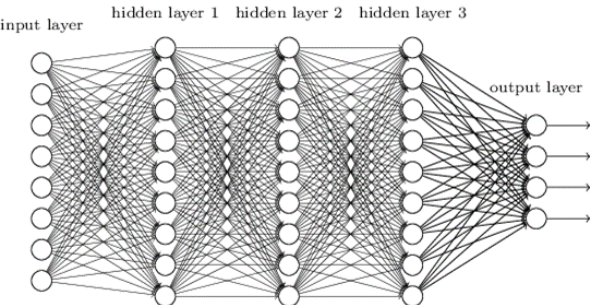
\includegraphics[width=0.7\textwidth]{images/deepnn}}
	\caption{A deep neural network with three hidden layers}
	\label{fig:deepl}
\end{figure}

Deep Neural Networks have been investigated for decades, but training deep networks consistently yielded poor results, until very recently. It was observed in many experiments that deep networks are harder to train than shallow networks, and that training deep networks often get stuck in apparent local minima (or plateaus) when starting with random initialization of the network parameters.

It was discovered, however, that better results could be achieved by pre-training each layer with an unsupervised learning algorithm \cite{hinton2006fast}. In 2006, \citeauthor{hinton2006fast} obtained good results using Restricted Boltzmann Machines (RBM) (a generative model) to perform unsupervised training of the layers \cite{hinton2006fast}. The goal of this training was to obtain a model that could capture patterns in the data, similarly to a feature descriptor, not using the dataset labels. The weights learned by this unsupervised training were then used to initialize neural networks. 

\indent Similar results were reported using auto-encoders for training each layer in \cite{bengio2007greedy}. These experiments identified that layers could be pre-trained one at a time, in a greedy layer-wise format. After the layers are pre-trained, the learned weights are used to initialize the neural network, and then the standard back-propagation algorithm (explained in Section~\ref{subsec:bp}) is used for fine-tuning the network. The advantage of unsupervised pre-training was demonstrated in statistical comparisons \cite{bengio2007greedy}, until recently when deep neural networks trained in a full supervised manner (using labeled data) started to register similar results in some tasks like object recognition. \citet{ciresan2012multi} demonstrated that properly trained deep neural networks (under full supervision) are able to achieve top results in many tasks, although not denying that pre-training might help, especially in cases were little data is available for training, or when there are massive amounts of unlabeled data. On the task of image classification, the best published results use a particular type of architecture called Convolutional Neural Network, which is described in below.



\section{Convolutional Neural Networks}
\label{sec:cnn}
Convolutional Neural Networks are a specialized kind of neural network for processing data that has a known grid-like topology such as image data which can be thought of as a 2D grid of pixels. CNNs are simply neural networks that use convolution in place of general matrix multiplication in at least one of their layers \cite{Goodfellow-et-al-2016-Book}. This type of network was used to obtain state-of-the-art results in the CIFAR-10 object recognition task \cite{ciresan2012multi}, and more recently in more challenging tasks such as the ImageNet Large Scale Visual Recognition Challenge \cite{russakovsky2015imagenet}. For both tasks, the training process benefited from the significant speed-ups on processing using modern GPUs (Graphical Processing Units), which are well suited for the implementation of convolutional networks.


Essentially, CNNs combine three architectural ideas to ensure some degree of shift and distortion invariance of local receptive fields, shared weights (or weight replication), and, sometimes, spatial or temporal sub-sampling \cite{lecun2010convolutional}. We are going to explain these basic ideas of CNN while introducing the main components that compose the main body of any CNN architecture.

\subsection{Convolutional Layer} 
\label{convlayer}
Each unit of a convolutional layer receives inputs from a set of units located in a small neighborhood in the previous layer. With local receptive fields, neurons can extract elementary visual features such as oriented edges, end-points and corners. These features are then combined by the higher layers \cite{lecun2010convolutional}. In addition, elementary feature detectors that are useful on one part of the image are likely to be useful across the entire image. This knowledge can be applied by forcing a set of units, whose receptive fields are located at different places on the image, to have identical weight vectors \cite{williams1986learning}. The outputs of such a set of neurons constitutes a \textit{feature map}. At each position, different types of units in various feature maps compute distinct types of features. Figure~\ref{fig:cnnsample} presents a convolutional layer functionality during forward propagation. 

\begin{figure}[H]
	\centering
	{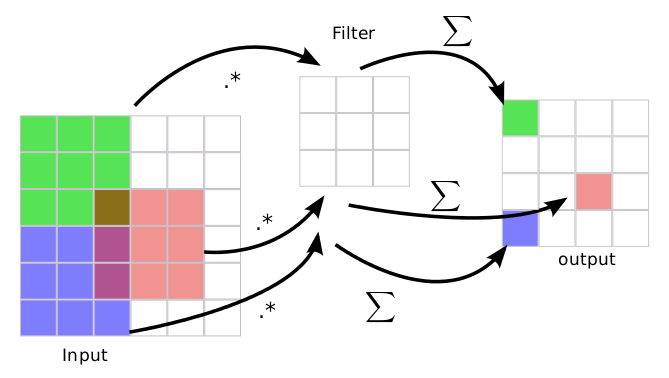
\includegraphics[width=0.7\textwidth]{images/conv}}
	\caption{The forward propagation phase of a convolutional layer}
	\label{fig:cnnsample}
\end{figure}
 
A sequential implementation of this process, for each feature map, would be to scan the input image with a single neuron that has a local receptive field, and to store the states of this neuron at corresponding locations in the feature map \cite{lecun2010convolutional}. \\
\indent Units in a feature map are constrained to perform the same operation on different parts ot the image. A convolutional layer is usually composed of several feature maps (with different weight vectors), so that multiple features can be extracted at each location. 

\noindent More formally, the definition of a 2D convolution is formulated in equation~\ref{eq:convf}. It is the
application of a discrete convolution of the inputs $y^{l-1}$ with a filter $w^{l}$ , adding a bias $b^{l}$, followed by the application of a non-linear function $\sigma$:

\begin{equation}
y_{rc}^{l} =  \sigma \sum_{i=1}^{F_r}\sum_{j=1}^{F_c}  y_{(r+i-1)(c+j-1)}^{l-1} (w_{ij}^{l} + b^{l})
\label{eq:convf}
\end{equation}

In this equation, $y_{rc}^{l}$ is the output unit at \{r, c\}, $F_r$ and $F_c$ are the number of rows and columns in the 2D filter, $w_{ij}^{l}$ is the value of the filter at position \{i, j\},  $y_{(r+i-1)(c+j-1)}^{l-1}$ is the value of input to this layer, at position \{r + i - 1, c + j - 1\}, and $b^{l}$ is the bias term.

The equation above is defined for all possible applications of the filter, that is, for $r~\in \{1, ..., X_r - F_r + 1\}$ and $c \in \{1, ..., X_c - F_c + 1\}$, where $X_r$ and $X_c$ are the number of rows and columns in the input to this layer. The convolutional layer can either apply the filters for all possible inputs, or use a different strategy. Mainly to reduce computation time, instead of applying the filter for all possible \{r, c\} pairs, only the pairs with distances are used, which is called the \textit{stride}. A stride, s = 1, is equivalent to apply the convolution for all possible pairs, as defined above. 

\noindent The inspiration for convolutional layers originated from models of the mammal visual system. Modern research in the physiology of the visual system found it consistent with the processing mechanism of convolutional neural networks, at least for quick recognition of objects \cite{bengio2009learning}. Although being a biological plausible model, the theoretical reasons for the success of convolutional networks are not yet fully understood. One hypothesis is that the small fan-in of the neurons (i.e. the number or input connections to the neurons) helps the derivatives to propagate through many layers - instead of being diffused in a large number of input neurons \cite{nips}.

\subsubsection{Weight Sharing}

Weight sharing refers to having several connections controlled by a single parameter (weight). Weight sharing can be interpreted as imposing equality constraints among the connection strengths. An interesting feature of weight sharing is that it can be implemented with very little computational overhead \cite{lecun1989generalization}. The weight sharing technique has an interesting side effect of reducing the number of free parameters, thereby the capacity of the machine and improving its generalization ability \cite{lecun2010convolutional}.



\subsection{Pooling/Sub-sampling Layer}
\label{poolinglayer}
Once a feature is detected, its' exact position becomes less important as long as its' approximate position relative to other features is preserved. Furthermore, as the dimensionality of applying a filter is equal to the input dimensionality, we would not be gaining any translation invariance with these additional filters. We would be stuck doing pixel-wise analysis on increasingly abstract features. In order to solve this problem, a \textit{sub-sampling} layer is introduced.

 Sub-sampling, or down-sampling, refers to reducing the overall size of a signal. In many cases, such as audio compression for music files, sub-sampling is done simply for size reduction. But in the domain of 2D filter outputs, sub-sampling  can also be thought of as reducing the sensitivity of the output to shifts and distortions.

One of the most applied sub-sampling methods used in \cite{lecun1995comparison}, is known as \textit{max-pooling}. Equation ~\ref{eq:pool} presents te formulation of a max-pooling layer. 

\begin{equation}
y_{rc}^{l} =  \max_{i,j\in\{0,1,...,m\} }  y_{(r+i-1)(c+j-1)}^{l-1}
\label{eq:pool}
\end{equation}
In this equation, $y_{rc}^{l}$ is the output for index \textit{{r, c}}, \textit{m} is the size of the pooling area, and $y_{(r+i-1)(c+j-1)}^{l-1}$ is the value of the input at the position \{r + i - 1, c + j - 1\}.


 
This involves splitting up the matrix of filter outputs into small non-overlapping grids (the larger the grid, the greater the signal reduction), and taking the maximum value in each grid as the value in the reduced matrix. A schematic of max-pooling is depicted in figure~\ref{fig:pooling}. Similarly for the convolutional layer described above, instead of generating all possible pairs of \{i, j\}, a \textit{stride, s,} can be used. In particular, a stride s = 1 is equivalent to using all possible pooling windows, and a stride s = m is equivalent of using all non-overlapping pooling windows.
\begin{figure}[H]
	\centering
	{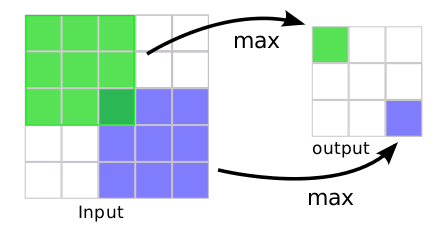
\includegraphics[width=0.5\textwidth]{images/pooling}}
	\caption{The forward propagation phase of a pooling layer with stride equal to 1.}
	\label{fig:pooling}
\end{figure}
 
\citet{scherer2010evaluation} evaluated different pooling architectures, and note that the max-pooling layers obtained the best results. Pooling layers add robustness to the model, providing a small degree of translation invariance, since the unit activates independently on where the image feature is located within the pooling window \cite{bengio2013deep}. Empirically, pooling has demonstrated to contribute to improved classification accuracy for object recognition \cite{lecun1989backpropagation}.


\subsection{Local Response Normalization}
\label{lrnlayer}
ReLU have the desirable property that they do not require input normalization to prevent them from saturating. If at least some training examples produce a positive input to a ReLU, learning will happen in that neuron. However, we still find that \textit{local response normalization}(LRN) scheme aids generalization. This sort of response normalization implements a form of lateral inhibition ( the capacity of an excited neuron to reduce the activity of its neighbors) inspired by the type found in real neurons, creating competition for big activities amongst neuron outputs computed using different kernels \cite{krizhevsky2012imagenet}. Figure~\ref{fig:lrns} illustrates local response normalization in a CNN. 
\begin{figure}[H]
	\centering
	{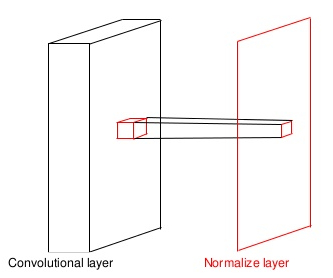
\includegraphics[width=0.5\textwidth]{images/lrn}}
	\caption{Local response normalization in a CNN after the convolution layer.}
	\label{fig:lrns}
\end{figure}

More formally, the activity $a_{x,y}^{i}$ of a neuron in bank \textit{i} at position \textit{(x,y)} in the topographic organization\footnote{The cerebral cortex of mammals primarily consists of a set of brain areas organized as topographic maps. These maps contain systematic two-dimensional representations of features relevant to sensory, motor, and/or associative processing, such as retinal position, sound frequency, line orientation, or sensory or motor motion direction \cite{patel2014topographic}.} is divided by:
\begin{equation}
\centering
\Bigg( 1+ \alpha \sum_{j=i-N/2}^{i+N/2} (a_{x,y}^{j})^{2} \Bigg)
\end{equation}
where the sum runs over \textit{N} " adjacent " banks of neurons at the same position in the topographic organization. The ordering of the bank is arbitrary and determined before training begins. The constants \textit{N}, $\alpha$ and $\beta$ are hyper-parameters whose values are determined using a validation set.

In other words, we can think of it as helping sharpening the response. Instead of carrying multiple ambiguous representation of a patch, it pushes the network to commit more towards a specific representation, freeing resources to analyze it better.

\indent This scheme bears some resemblance to the local contrast normalization scheme proposed by \citeauthor{jarrett2009best} in \cite{jarrett2009best} which has led to error rate reduction in \cite{krizhevsky2012imagenet} and \cite{hinton2012improving}. 

\subsection{Fully Connected/Inner Product Layer}

Finally, after several convolutional and max pooling layers, the high-level reasoning in the neural network is done via \textit{fully connected layers} (FC/IP). A fully connected layer takes all neurons in the previous layer (be it fully connected, pooling, or convolutional) and connects it to every single neuron it has. Fully connected layers are not spatially located anymore (you can visualize them as one-dimensional), so there can be no convolutional layers after a fully connected layer. 






\newpage
\chapter{State of the Art Review}
\label{sec:stateoftheart}

In this chapter, we present a review of state-of-the-arts regarding synthetic data generation for deep neural networks to be applied for learning to count tasks. We introduce a summary of cutting-edge research studies from two aspects. First we succinctly review the background of generating synthetic data for different problems, and then a short history of feature detection algorithms will be alluded.

\section{Synthetic Data Generation} 

The main purpose of generating synthetic datasets has been to protect the privacy and confidentiality of the actual data \cite{yao2015synthetic,phua2010comprehensive}, since it does not hold any personal information and cannot be traced back by any individual. Problems such as fraud detection \cite{phua2010comprehensive}, or health care \cite{yao2015synthetic}, are normally tackled by the use of synthetic data. These datasets might seem to be "made up" data, however, there are certain algorithms and generators that are designed to create realistic data \cite{yao2015synthetic,arasu2012synthetic}. 

In addition, synthetic data are often used to meet specific needs or certain conditions that may not be found in the original, real data. This can be useful when designing any type of system because the synthetic data are used as a simulation or as a theoretical value, situation, etc. For example, in \cite{hofmeyr1998intrusion}, the authors introduce a method for detecting intrusions where the experiment is done using synthetic data. This data is a representation of the authentic data and may include intrusion instances that are not found in the authentic data. The synthetic data allows the software to recognize these situations and react accordingly.

Furthermore, in computer vision, the use of synthetic images has a longstanding history, as in \citeyear{cappelli2000synthetic}, \citealt*{cappelli2000synthetic} presents an approach to synthetic fingerprint generation on the basis of some mathematical models that describe the main features of real finger prints. The process of generating finger prints follows a simple course (as shown in Figure~\ref{finger}). First, a fingerprint shape, a directional map and a density map are generated separately; then these three features are combined to obtain a fingerprint pattern, which is finally more realistic by adding noise.

\begin{figure}[H]
	\centering
	{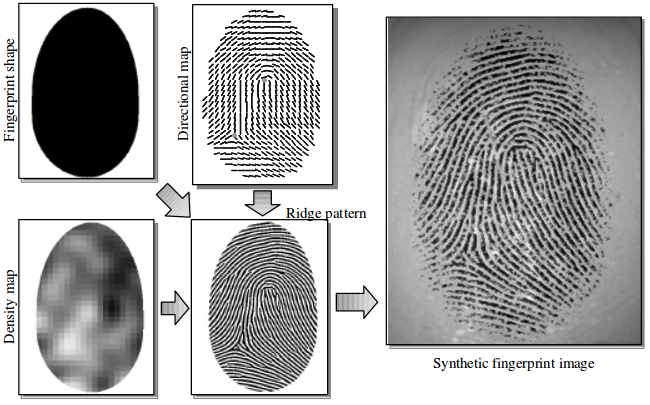
\includegraphics[width=0.5\textwidth]{images/finger}}
	\caption{The basic idea of the synthetic fingerprint generation approach \cite{cappelli2000synthetic}.}
	\label{finger}
\end{figure}


More recently, after the success of deep convolutional neural networks in various vision tasks concerning object detection or classification, generation and use of synthetic datasets has been frequently considered. As a viable alternative to complement the real data, synthetically generated training sets can remarkably improve the performance of DCNNs when the real data is limited \cite{eggert2015benefit,hu2016frankenstein,jaderberg2014synthetic,gaur2015generation}. For example, in \cite{eggert2015benefit}, synthetic images are generated to be fed to a DCNN in order to learn how to detect company logo in the absence of a large training set. In order to generate the images, first they select a random perspective transform and warp both image and mask accordingly. Then, they modify the color of the warped image to provide a larger visual variety. Later, the logo is randomly blurred by convolution with a Gaussian kernel (with different $\sigma$ values) to simulate different scales. Finally, the background is removed of the logo and the warped and color-modified logo into a new image which contains no logo. This process is shown in figure~\ref{cocacola}.

\begin{figure}[H]
	\centering
	{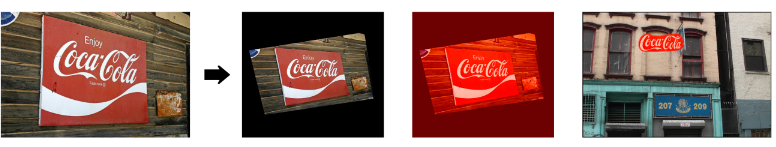
\includegraphics[width=0.9\textwidth]{images/cocacola}}
	\caption{An example of synthetically generated images in \cite{eggert2015benefit}. Starting from a base image, a random perspective transform is applied,  followed by gaussian blur (not shown),  color augmentation (exaggerated for viewing purposes) and background replacement.}
	\label{cocacola}
\end{figure}

 
%Furthermore, synthetic data have been applied by recent learning algorithms as a viable alternative to complement the real data where the real data is not publicly available, or quite difficult to collect \cite{hu2016frankenstein}. These datasets are generated at a high realistic state and preserve high levels of accuracy compared to the original data. For instance, in \cite{gaur2015generation}, the authors improve the performance by creating additional synthetic training data due to the lack of real dataset. Moreover, \citealt*{jaderberg2014synthetic} introduces a framework for natural scene text recognition solely by training deep convolutional neural network with synthetically generated and labeled data.

%\noindent The use of synthetic data has a longstanding history in computer vision and more specifically for object detection problems. For example, \cite{shotton2013real} used synthetic dataset to propose a method for human pose prediction while In \cite{rematas2014image}, the author proposed a technique to improve novel-view synthesis for images using the structural information\footnote{Structural information theory (SIT) is a theory about human perception and in particular about visual perceptual organization, which is the neuro-cognitive process that enables us to perceive scenes as structured wholes consisting of objects arranged in space.} from 3D models. 
 
%After the success of deep learning algorithms in solving various problems in computer vision by obtaining cutting-edge results, generate and use of synthetic data has been considered for training different learning algorithms as a viable alternative to complement the real data \cite{gaur2015generation,jaderberg2014synthetic}. In particular, convolutional neural networks have been used to learn from synthetically created datasets \cite{rematas2014image,gaur2015generation,jaderberg2014synthetic}. 
Moreover, As one of the most recent approaches, \citeauthor*{segui2015learning} in \cite{segui2015learning} proposed synthetic data generation to counter lack of data issue for learning to count the number of objects in images using deep convolutional neural networks. In their work, they took advantage of existent unlabeled and labeled datasets to generate realistic synthetic images representative of the actual images. The authors introduce two counting problems, counting number of even-digits in images, and counting the amount of pedestrians in a walkway. In the former problem, they incorporated real labeled hand-written digits to make images with up to five digits in the image. Figure~\ref{digped} depicts an example of generated images in \cite{segui2015learning}.


\begin{figure*}[h!]
    \centering
    \begin{subfigure}[t]{0.5\textwidth}
        \centering
        {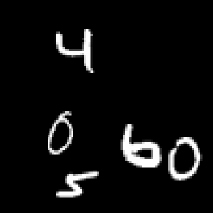
\includegraphics[width=0.6\textwidth]{images/digdigdig}}
        \caption{Synthetic image for even digits counting problem.}
    \end{subfigure}%
    ~ 
    \begin{subfigure}[t]{0.5\textwidth}
        \centering
        {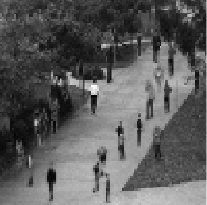
\includegraphics[width=0.6\textwidth]{images/pedpedped}}
        \caption{Synthetic image for counting the number of pedestrians.}
    \end{subfigure}
    \caption{An example of synthetically generated images by \citealt*{segui2015learning}.}
    \label{digped}
\end{figure*}

For the latter one, they used an unlabeled set of images (video frames) of pedestrians in a walkway. The creation of images is as follows: First, a simple background subtraction technique is used. Then a Gaussian filter is applied across the backgrounds to smooth out motion effects. Afterwards, the candidate pedestrians are extracted subtracting the background. Background noise and imperfect shapes are handled using mathematical morphology operators. At last, new artificial images are synthesized by means of a composition of backgrounds and pedestrians' sub-images. Each image contains up to 25 pedestrians \cite{segui2015learning}. After generating these synthetic datasets, they used deep convolutional neural networks to learn the object features in order to count the number of objects present in the images.     
  
\section{Feature Detection Algorithms} 
\label{fda}
Counting the number of an object of interest in an image can be approached from two different perspectives: either training an object detector, or training an object counter \cite{segui2015learning}. In the field of object detection, numerous works have been previously proposed \cite{davies1995crowd, kong2005counting, marana1998efficacy}. Most of these research works follow a taxonomy which consists of three paradigms underneath to count the objects \cite{chan2008privacy}:

\begin{enumerate}
	\item Object detection methods, which were based on boosting motion and appearance features, Bayesian model-based segmentation, integrated top-down and bottom-up processing.
	\item Visual feature trajectory clustering. This paradigm counts objects by identifying and tracking visuals over a  time period. Feature trajectories with coherent motion are then clustered and the number of clusters is the estimate of the number of objects. 

	\item Feature-based regression. These methods usually work by first, subtracting the background, second, measuring various features of the foreground pixels such as total area, edge count, or texture; and finally estimating the objects' density or objects' count by a regression function, e.g. linear, piece-wise linear, or neural networks. 

	\indent In recent years, feature-based regression has also been applied to outdoor scenes. For example, \citealt{kong2005counting} apply neural networks to the histograms of foreground segment areas and edge orientations. \citealt{dong2007fast} estimate the number of people in each foreground segment by matching its shape to a database containing the silhouettes of possible people configurations, but that would be only applicable when the number of people in each segment is small (empirically, less than 6) \cite{chan2008privacy}.  
\end{enumerate} 
By reason of the fact that almost all the above algorithms detect the whole objects in an image (e.g. whole pedestrians), these methods have moderate performance in very noisy or crowded images with significant occlusion, \citealt*{wu2005detection, lin2001estimation}, introduced methods to address this issue. \citealt*{wu2005detection} proposed \textit{edgelet features} (an edgelet is a short segment of line or curve) as new type of silhouette oriented features to deal with the problem of detecting individuals in crowded still images. %Respectively in \cite{lin2001estimation}, \citeauthor*{lin2001estimation} used \textit{Accumulated Mosaic Image Difference(AMID)} method to extract crowd areas having irregular motion. 

\indent As a similar line of work in the course of object counting and more specifically crowd counting, in \cite{rabaud2006counting, brostow2006unsupervised, leibe2007coupled}, different object tracking approaches were taken to detect and count moving objects in the scene. However, the deployment of these vision surveillance technologies are invariably met with skepticism by society at large, given the perception that they could be used to infringe individuals' privacy rights (through tracking individuals as objects in order to count their multiplicity). While a number of methods that do not require explicit detection or tracking have been previously proposed \cite{paragios2001mrf, cho1999neural, regazzoni1996distributed, davies1995crowd, kong2005counting, marana1998efficacy, dong2007fast}, they have not fully established the viability of the privacy-preserving approach \cite{chan2008privacy}. The tension of privacy-preserving is common in all areas of data-mining \cite{vaidya2006privacy, verykios2004state}. 

In order to tackle privacy preserving issue, \citealt*{chan2008privacy} presented a novel approach with no explicit object segmentation or tracking to estimate the number of people moving in each direction(towards and away from camera) in a privacy-preserving manner. An outline of the crowd counting system appears in figure~\ref{fig:ucsd}:
\begin{figure}[H]
	\centering
	{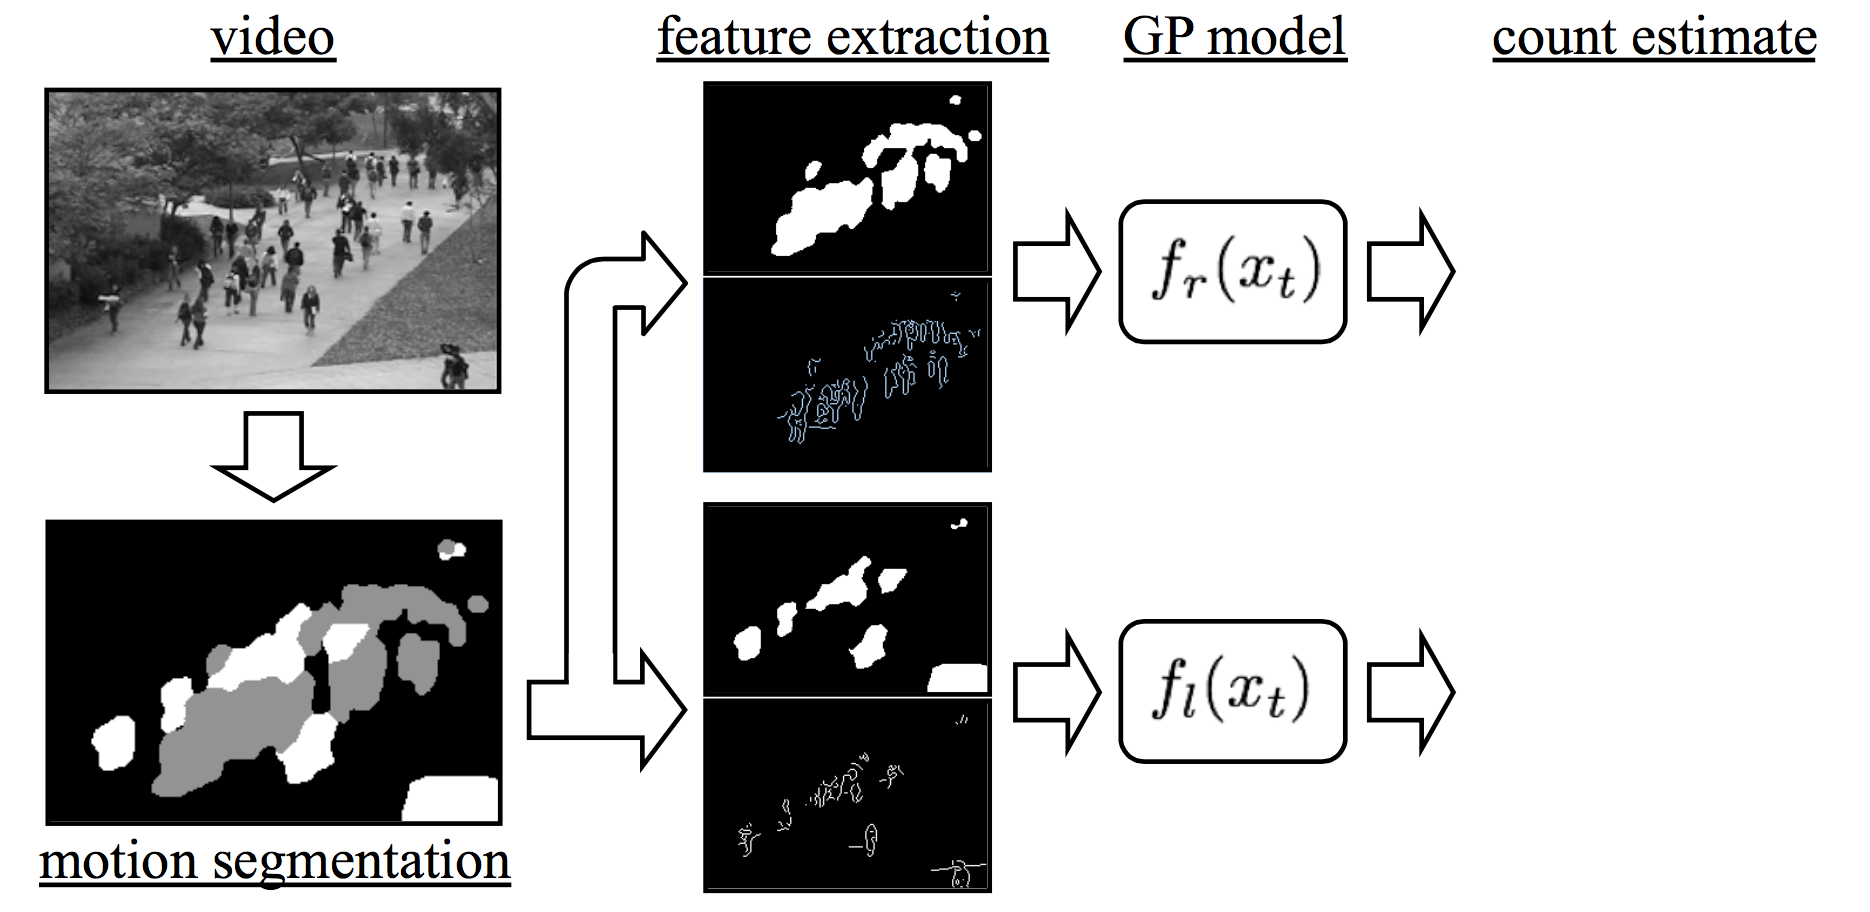
\includegraphics[width=0.8\textwidth]{images/ucsdOutline}}
	\caption{Crowd counting system: the scene is segmented into crowds with different motions. Normalized features that account for perspective are extracted from each segment, and the crowd count for each segment is estimated with a Gaussian process \cite{chan2008privacy}.}
	\label{fig:ucsd}
\end{figure}

\citeauthor*{chan2008privacy} used a mixture of \textit{dynamic textures}\footnote{Dynamic textures are sequences of images of moving scenes that exhibit temporal regularity, intended in a statistical sense, like sea-waves, smoke, foliage, whirlwind but also talking faces, traffic scenes etc.} \cite{doretto2003dynamic, chan2008modeling} to divide the video frames into regions containing moving pedestrians in different directions. When adopting mixture of dynamic textures, the video is represented as collection of spatio-temporal patches which are modeled as independent samples from mixture of dynamic models \cite{doretto2003dynamic}. The mixture model is learned through Expectation-Maximization(EM) algorithm \cite{chan2008modeling}. Video locations are then scanned sequentially, a patch is extracted at each location, and assigned to the mixture component of largest posterior probability. The location is declared to belong to the segmentation region associated with that component  \cite{chan2008privacy}. The resulting segmentations of their work are illustrated in figure~\ref{fig:segUcsd}:
\begin{figure}[H]
	\centering
	{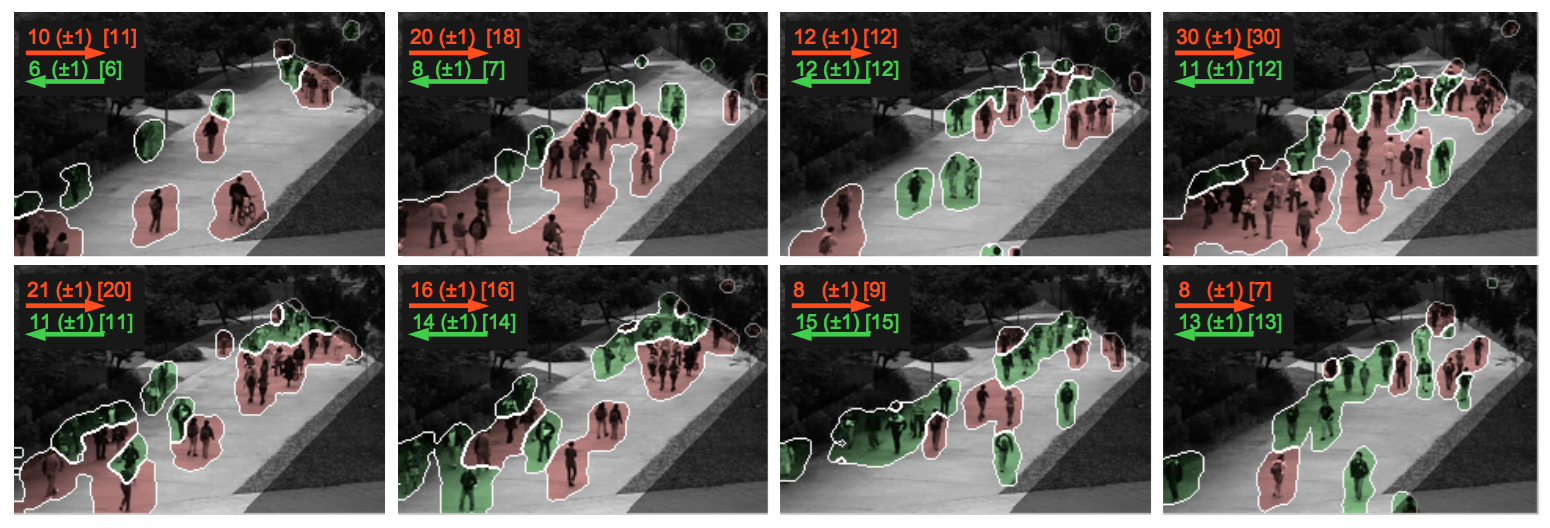
\includegraphics[width=0.9\textwidth]{images/segUcsd}}
	\caption{Crowd counting results: The red and green segments are the “away” and “towards” crowds. The estimated crowd count for each segment is in the top-left, with the (rounded standard-deviation of the GP) and the ground-truth. The Region Of Interest (the area in the walkway in which the pedestrians are counted and labeled) is also highlighted \cite{chan2008privacy}.}
	\label{fig:segUcsd}
\end{figure}

After segmenting the moving pedestrians, extracting features from the video segments is done at three phases:
\begin{itemize}
	\item Segment features to capture segment shape and size. Features such as area, perimeter, perimeter edge orientation and perimeter-area ratio. 
	\item Internal edge features contained in a crowd segment are a strong about the number of pedestrians in the segment \cite{davies1995crowd, kong2005counting}. For instance, total edge pixels and edge orientation. 
	\item Texture features which are based on gray-level co-occurrence matrix\footnote{Co-occurrence matrix is a matrix that is defined over an image to be the distribution of co-occurring values at a given offset.} (GLCM) (see  \cite{haralick1973textural} for more details) were applied for image patches classification into 5 classes of crowd density in \cite{marana1998efficacy}. Due to the task similarity, \citeauthor*{chan2008privacy} adopted a similar set of measurements for counting the number of crowd in each segment, and computed texture properties like homogeneity, energy and entropy. 
\end{itemize} 
%\cite{williams2006gaussian}
Having segments' features extracted, a Gaussian Process\footnote{Gaussian Process is a statistical distribution in which the occurrence of observations happen in a continuous domain such as time or space. The distribution of a GP is a distribution over functions in a continuous domain.} (GP)  was used to regress feature vectors to the number of people per segment. The GP defines a distribution over functions, which is “pinned down” at the training points \cite{chan2008privacy}. Since the classes of function that GP can model is directly dependent on the selected kernel function, they combined the linear and the squared-exponential (RBF) (see \cite{chang2010training, vert2004primer, shashua2009introduction} for more details) kernels, \textit{i.e.}
\begin{equation}
\centering k(x_p, x_q) = \alpha_1(x_p^{T}x_q+1) + \alpha_2e^{\frac{-\|x_p-x_q\|^2}{\alpha_3}} + \alpha_4\delta(p,q)     
\end{equation}
The linear component of the kernel captures the dominant trend of many features which is linear (\textit{e.g.} segment area), while the RBF component models local non-linearities that arise from a variety of factors, including occlusion, segmentation errors and pedestrian configuration (\textit{e.g.} spacing within a segment) \cite{chan2008privacy}. 
  
For this experiment, they collected an hour of video from a stationary digital camera. The first 2000 frames of the videos were annotated as ground-truth. Moreover, a region-of-interest (ROI) was defined on the walkway (see figure~\ref{fig:segUcsd}), and the traveling directions (away from or towards the camera) and visible center of each pedestrian was annotated. Then the video was split into a training set, for learning the GP, and a test set for validation. The training set contains 800 frames, between frame 600 and 1399, with the remaining 1200 frames held out for testing. This dataset is available to the vision community \cite{chan2008privacy}.

%The obtained results for crowd counting in  \cite{chan2008privacy} are expressed as both mean-squared-error (MSE) and mean-absolute-error (MAE) between the estimate and ground-truth. 
Although they obtained reasonable results in a privacy-preserving manner, their worked required exhaustive data annotations along with hand-crafting highly specialized image features that were dependent on the object class (pedestrians).  


%However, if the problem is tackled from the perspective of object counters and not object detectors, we only need to provide the number of object instances for each image sample and the result is typically a regressor\cite{lempitsky2010learning}.  

In order to save annotation efforts, different techniques were used to count objects. Multiple Instance Learning (MIL) \cite{foulds2010review} is a variation of supervised learning in which instances come in bags. These bags contain multiple samples. A bag is labeled positive if there is at least one example with the concept of interest, or labeled negative otherwise. The positive bag can be regarded as a set of attracting instances and the negative one as a set of repulsive instances. In large-scale computer vision, this approach is frequently found under the name of \textit{weakly supervised learning} \cite{weber2000unsupervised, fergus2003object}. There are different definitions for the term "weakly" in the literature. For instance, in \cite{dekel2009good}, it is a surrogate for the concept of noisy labels such as labels provided by different supervisors with distinct quality. However, in \cite{raykar2009supervised}, it is described for indicating imperfect annotation or even in \cite{wang2013weakly} for specifying only the presence of an object in an image. 

\indent Early works used weakly supervised learning in an instantiation of the MIL framework for inferring difficult to describe classes such as in \cite{todorovic2006extracting} where photometric, geometric, and topological features are recognized. More recently, several works, such as \cite{nguyen2009weakly}, explore the capacity of this technique for simultaneous localization and recognition. Another work using MIL framework was count-based multiple instance learning \cite{foulds2010review}. In count-based MIL the positive bag is composed of instances where the concept appears within the range of an interval. For example, the positive bag may contain images with 5 to 10 appearances of pedestrians. A major drawback of MIL framework is that even in count-based MIL the problem is casted as a binary task and they would not be applicable in projects where the exact number of objects in the image important. 

Furthermore, another approach to reduce the annotation tasks is done in \cite{flaccavento2011learning}, where the labeling process is decreased to dotting(pointing) and the counting process is addressed as image density estimation problem.  

Recently, with the success of CNNs in different vision tasks, object detection systems based on deep CNN have made groundbreaking advances on several object detection problems \cite{zhang2015improving, erhan2014scalable, girshick2014rich, he2015spatial, erhan2014scalable} which suggests the use of this technique to learn to count objects. Several advantages can be foreseen from this application, being the most important that of learning image features from samples instead of hand-crafting highly specialized image features that are dependent on the object class \cite{segui2015learning}. Moreover, CNN have shown their capacity of knowledge transfer for a number of tasks or the ability of simultaneously performing different tasks even when trained for only one \cite{zhou2014learning}. 

Following this line of work,  \citefullauthor{segui2015learning} in \cite{segui2015learning} proposed a novel approach for counting objects' representations using deep object features. In their work, objects' features are learned by a deep counting convolutional neural network and are used to understand the underlying representation. Their proposal lies in the middle of weakly supervised learning and fully supervised learning \cite{mohri2012foundations}. It is similar to weakly supervised learning because the location of the concept of interest is not given. Whereas, unlike fully supervised learning in which the object boundary or bounding box is given to the learning process, in their proposed architecture, only the multiplicity of the object is provided \cite{segui2015learning}.

To this end, they defined a counting problem for even digits and demonstrated that the internal representation of the network is able to classify digits in spite of the fact that during training, no direct supervision was provided. Moreover, they present preliminary results about a deep network that is able to count the number of pedestrians in a scene \cite{segui2015learning}. Figure~\ref{fig:santimnist} illustrates their proposal at a glance in the case of representing hand-written digits:
\begin{figure}[H]
	\centering
	{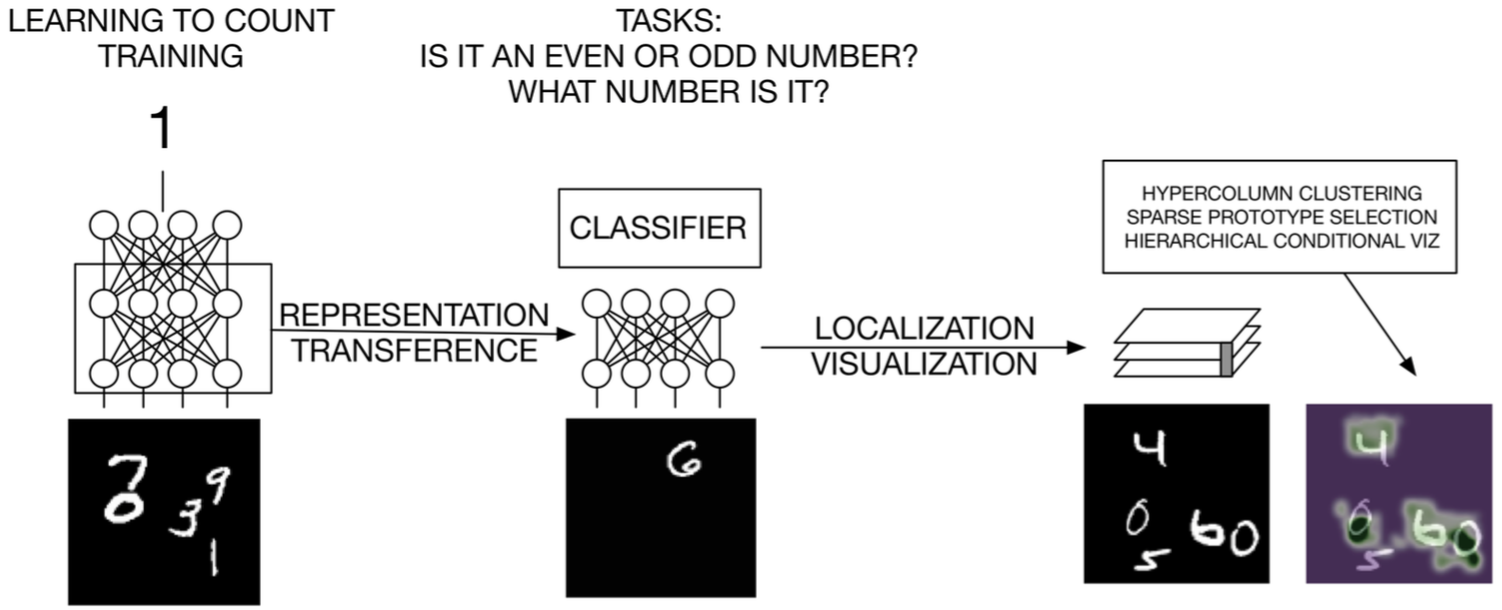
\includegraphics[width=0.9\textwidth]{images/santimnist}}
	\caption{Learning to count hand-written digits problem in which the features of a CNN that has been trained to count digits can be readily used for more specific classification problems and even to localize digits in an image \cite{segui2015learning}.}
	\label{fig:santimnist}
\end{figure}

In \cite{segui2015learning}, the main hypothesis is that the number of occurrence of objects in an image provide strong presentational information due to their possible discriminate appearance for a feature learning process to exploit. In order to verify this hypothesis, for both experiments, they considered networks of two or more convolutional layers (since CNNs instinctively handle feature learning \cite{lecun1989backpropagation}) consisting of convolutional filters, ReLU non-linearities, max-pooling layers and normalization layer, followed by one or more fully connected layers (regarding the impressive classification performance on different benchmark problems \cite{krizhevsky2012imagenet, Karpathy_2014_CVPR, ciresan2011flexible}) \cite{segui2015learning}. 

For learning to count in the hand-written digits domain, they synthetically created a set of one million images of size $100\times100$ including random digits from the MNIST database with maximum 5 digit per image and with no overlapping in the images. Obtaining accuracy of 93.8\% on the base network, along with results attained from training a support vector machine (SVM) with the representations learned on different layers of the network, validates this hypothesis that counting process can be considered as a surrogate to potentially extract or infer interesting object descriptors \cite{segui2015learning}. 

Additionally, for learning to count the number of pedestrians in a scene, they used UCSD pedestrian database \cite{chan2008privacy}. Once again, \citealt*{segui2015learning} created a set of 200.000 synthetic images each containing up to 25 pedestrians. The results in this scenario are encouraging and reinforce the feasibility of the proposal in front of counting problems. However, still there are some deficiencies that should be obviated. For instance, how would a model trained by synthetic dataset perform on real dataset and in a real world problem? Or would the model still be able to learn object representations in scaled-up and more complex scenarios?







\newpage
\chapter{Proposal}
\label{sec:proposal}
\noindent

This master thesis presents an analysis on the synthetic data generation procedure as a feasible alternative for lacking or missing real data, as well as proposes an application of deep convolutional neural networks for the task of counting objects in the images. The developed systems will address some of the issues common to other object detection algorithms. These issues include: 

%This master thesis proposes an application of deep CNNs to the task of counting objects in the image. The developed systems will address some of the issues common to other object detection algorithms. These issues include:
\begin{itemize}
	
	\item Obtaining poor results due to lack of data. 
	\item Painstaking hand-crafted image features which are highly dependent on the object class. 
	\item Scrupulous data annotation for manifold data. 
	\item Establishing the viability of a privacy-preserving approach. 
	\item Being prone to error in noisy or crowded scenes with a noticeable occlusion. 

\end{itemize} 
In addition, the state-of-the-art \cite{segui2015learning} technology lacks applicability for real-world counting problems due to being tested only on synthetic dataset.


The novelty of our approach compared to the state-of-the-art is that we present highly-realistic synthetic data generation algorithms for training DCNN. Consequently, by the use of these realistic datasets, we hypothesize that features learned by DCNN with synthetic dataset, are representative enough to count the number of object of interest in a real dataset. We tackle this task as a regression problem. 
To the best of our knowledge, the proposed work would be the first one in which a counting system trained with synthetic images is able to be incorporated in real-world similar counting problems.

Henceforth, in the rest of this chapter, we justify both our synthetic data generation process and our proposed methodology along with a comparison to state-of-the-art from different aspects including method selection and architecture.   

%Henceforth, in the rest of this chapter, we justify our methodology along with a comparison to state-of-the-art from different aspects including method selection, architecture, dataset and its application.   

\section{Datasets} 

In this section, starting with a short review of data for DCNN in computer vision, we express a succinct reasoning on the benefit of synthetically generated datasets we used in our experiments. Later on, in the implementation section, the specifications and preprocessing phases regarding each dataset will be described in details. 

%In this section, starting with a short review of data for DCNN in computer vision, we express a succinct reasoning about the datasets we used in our experiments. Later on, in the implementation section, the specifications and preprocessing phases regarding each dataset will be described in detail. 

In spite of remarkable  performance of DCNN in some simple recognition benchmarks \cite{cirecsan2011convolutional, ciresan2015multi, wan2013regularization, cirecsan2012multi}, until recently the models' performances were poor at more complex datasets  \cite{griffin2007caltech} due to lack of labeled input samples to train the network parameters with. It was with the creation of ImageNet \cite{deng2009imagenet} and GPU implementation \cite{krizhevsky2012imagenet} ($50\times$ speedup over CPU) that efficiency of deep CNN in vision tasks became crystal clear.

However, there are still many areas such as crowd counting in which large training set is either missing or not publicly available due to privacy-preserving policies. In these types of problems, synthetic data generation can be a well-suited surrogate for the missing actual data.  Access to unsupervised images and also the existence of powerful image processing tools enable us to create highly realistic images. Hence, in this work we propose two synthetically created datasets related to proposed learning to count problems for the application of deep convolutional neural networks. First learning to count even-digits dataset and then a set of images for counting the number of pedestrians present in the images.   

The proposed synthetic datasets facilitate the application of deep convolutional neural networks for problems concerning learning to count the number of object of interest. Moreover, in the case of counting the number of pedestrians, it preserves the individuals' privacy since the data is synthetic and not real (as explained in chapter~\ref{fda}, previous crowd counting approaches were somehow infringing individuals' privacy by using object tracking algorithms.). Consequently, the application of DCNNs lead to easier feature detection process and improvement of the system's performance. 

\subsection{Learning to Count Even-digits Dataset}

In this study, we introduce a synthetic dataset using MNIST dataset. The MNIST database of handwritten digits, has a training set of 60,000 examples, and a test set of 10,000 examples. The digits have been size-normalized and centered in a fixed-size image \cite{lecun1999mnist}. In the MNIST dataset, each image contains one hand-written digit of dimensions $28\times28$. Figure~\ref{fig:mnistimages} shows a selection of MNIST dataset images.

\begin{figure}[H]
	\centering
	{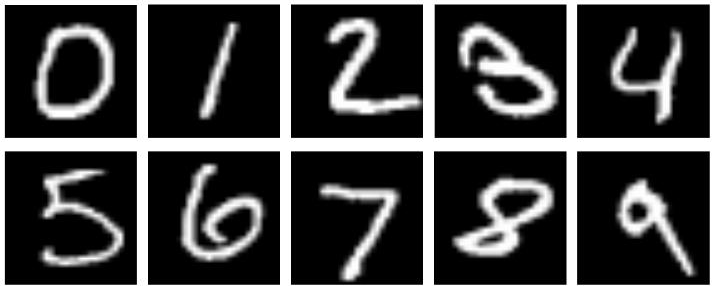
\includegraphics[width=0.7\textwidth]{images/mnistall}}
	\caption{A selection of MNIST images of hand-written digits.}
	\label{fig:mnistimages}
\end{figure}


\noindent For the first empirical experience in our work, we created a large set of images each containing up to 15 MNIST digits. Images are automatically labeled with the number of even digits in each image. Using this dataset, we can examine the digits' representations learned by our deep CNN are not dependent on the specific task we are dealing with. It is done by using our model's learned features for other tasks and analyze the results. 

\subsection{Synthetic Crowd Counting Dataset}

As we needed a large dataset to train all the parameters of our model for the second task, counting the number of pedestrians, we synthetically created a large dataset of pedestrians in a walkway with maximum 29 people in each image. Achieving success on crowd counting system using CNN on our synthetic dataset, we save enormous amount of time for data annotation and feature detection. 

\subsection{UCSD Crowd Counting Dataset}

However, we need our model to perform well in practice rather than in theoretical experiments. Therefore, we used UCSD crowd counting dataset \cite{chan2008privacy} to validate the performance of our model on it and also make a comparison with their system in \cite{chan2008privacy} to see if we can obtain better results while decreasing feature extraction and labeling efforts. In addition, if we succeed to attain reasonable results on the real UCSD dataset, we have overcome one of the main restrictions of deep learning algorithms usage, which is the necessity for the existence of large amount of data.     


\section{Method Selection}

For a long time in Computer Vision, there has been a prevailing paradigm in which we have a set of feature descriptors such as SIFT \cite{lowe1999object}, HOG \cite{dalal2005histograms}, SURF \cite{bay2006surf}, and others that can be extracted from the image with possible higher level feature building (High-level feature detection algorithms are more in tune with the way we detect objects in real life), following by a classifier like Support Vector Machines (SVM) \cite{vapnik1964note, boser1992training}. In fact, for the most part, these features are not learned, but hand-crafted by some vision experts. However, they do indeed demonstrate a decent performance. For instance, in one of the most successful works in object detection \cite{felzenszwalb2010object}, the author essentially introduces a linear classifier on top of HOG features, or regarding classification approaches that work quite well, \citeauthor{yu2010object} use all manners of features (HOG, SIFT, Color SIFT, etc) extracted from the images and consequently obtain impressive results. 

\indent The analysis of these works leads to the question of what we should focus on in order to improve the vision systems accuracy. Should we try to enhance classifiers, should we increase the amount of data or we should rather provide finer features? \citeauthor*{parikh2010role} in \cite{parikh2010role} analyze the role of features by taking some of the quite successful past deformable models\footnote{Deformable models are curves or surfaces defined within an image domain whose deformations are determined by the displacement of a discrete number of control points along the curve \cite{xu2000image}.}, and replace some components of them with humans. They present identical learning tasks \textit{i.e.} the same feature representation and the same training data to machines and humans which allows drawing a comparison between the two. The author concludes that features are the main factor contributing to superior human performance.

Furthermore, in \cite{gehler2009feature}, the authors compared 39 different learning kernels with various combination of features to see which kernel outperforms the rest and how it should be weighted. Although they attained a big improvement over the existing methods, the analysis of their results shows that the gain they obtained from the learning operators is not as dramatic as the improvement they achieved from the features itself. 

\indent Therefore, since the features are providing the biggest impact in these algorithms, if we improve those features, we can acquire better algorithms. The difficulty of feature improvement and high cost of numerous feature computations on each image brought us into the application of deep learning in order to learn the features themselves rather than hand-crafting them. 

In deep learning techniques, we essentially have a hierarchy of feature extractors which attempts to model high-level abstractions in data \cite{deng2014deep, bengio2009learning, bengio2013representation, arel2010deep, schmidhuber2015deep}, where each layer of hierarchy extracts features from output of previous layer. Designing such trainable feature extractors, we would be able to build a multi-stage model which goes all the way from image pixels up to a high-level feature vector which we can be fed to a standard classifier. 

Thus, from the family of DL, we select deep CNNs due to their capacity of knowledge transfer for a number of tasks and also the ability for performing different tasks simultaneously, even when it has been trained for only one task \cite{zhou2014learning}. Moreover, compare to other methods, DCNN benefit from the powerful speed-ups on GPU which is fit for implementation of DCNN. 

Furthermore, DCNN was used to achieve state-of-the-art results in CIFAR-10 object recognition task \cite{cirecsan2012multi}, in \cite{russakovsky2015imagenet}, the training process was done on GPU, and a great success in many other recent vision problems \cite{cirecsan2011convolutional, ciresan2015multi, wan2013regularization}. All these features and advantages of CNN assured us to choose convolutional neural networks as our proposed method

\section{Architecture}

With their long heritage, the origins of CNN trace back to \cite{hubel1962receptive} where first simple cells (brain cell) detect local features and afterwards, complex cells pool the outputs of simple cells within a retinotopic\footnote{Retinotopy is the mapping of visual input from the retina to neurons, particularly those neurons within the visual stream. For clarity, 'retinotopy' can be replaced with 'retinal mapping', and 'retinotopic' with 'retinally mapped}neighborhood (see \cite{hubel1962receptive} for more detailed explanation). Also, \citeauthor*{fukushima1975cognitron} in \cite{fukushima1975cognitron, fukushima1980neocognitron} introduced a similar architecture with filtering layers followed by pooling layers. However, the first deep CNN architecture was designed by \citealt{lecun1989backpropagation} who demonstrated that this kind of architecture can perform quite well for vision tasks like digit recognition. A schematic of \citeauthor{lecun1989backpropagation}'s proposed architecture has been depicted in figure~\ref{fig:lecun}

\begin{figure}[H]
	\centering
	{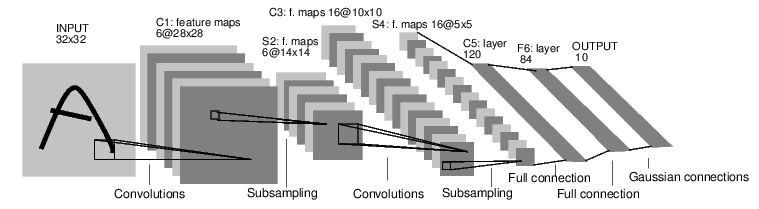
\includegraphics[width=1\textwidth]{images/lenetarch}}
	\caption{Deep CNN proposed by \citealt*{lecun1989backpropagation} for MNIST hand-written digits recognition problem.}
	\label{fig:lecun}
\end{figure}

Following the same structure of classical CNNs, in our architecture, the image pixels are fed to a convolutional layer, where relatively small filters (windows) shift over the image (not necessarily pixel by pixel, as a different stride can be taken) and produce feature maps. Since convolution is a linear operation, in order to make the model non-linear, feature maps are passed to rectified linear units (ReLU) \cite{nair2010rectified} which is applied to each element of the feature map independently. 

As discussed in chapter~\ref{sec:actfun}, ReLU is currently favored in the research community given the fact that it fastens the learning process by massively simplifying back propagation, and also avoids saturation issues (when the weighted sum is big, the output of the $\tanh$ or \textit{sigmoid} activation functions saturates and the gradient tends to zero. See \cite{hansen1990neural, amit1987statistical} for more details). 

\indent Thereafter, a max-pooling layer takes a special region of the obtained feature maps and takes the maximum pixel value as the strongest structure of that neighborhood (described in section~\ref{poolinglayer}). We chose Max-pooling since it tends to give more discrimination of the features \cite{boureau2010theoretical}. In our model we use \textit{spatial} pooling. However, depending on the problem we are trying to solve, pooling might be done within feature maps \cite{goodfellow2013maxout}. The main advantage of pooling layers in the architecture can be that it results in invariance to small transformations. In addition to that, as we go up in DCNNs, thanks to pooling, each of the units essentially has a larger receptive fields looking back the input so that at the top high-level layers, each unit looks at the entire scene.  

To improve the model performance, after each pooling layer in the proposed model, we used local response normalization layer (LRN) to apply a contrast normalization(explained in details in chapter ~\ref{lrnlayer}). This type of normalization was introduced and used for the first time in \cite{krizhevsky2012imagenet}. Empirically, using LRN in the architecture seems to help improving the results \cite{jarrett2009best, krizhevsky2012imagenet}. 

%%%In essence (explained in details in chapter ~\ref{lrnlayer}), LRN introduces a local competition between features, in a way that it picks a single location in the output and it looks at a special neighborhood around that location in the input. Then it computes the local mean in that region, weighs it by the Gaussian distribution, translates and makes it to corresponding vectors with local mean = 0 and local standard deviation = 1 (the chosen values are problem dependent; in our case, we chose $\mu = 0$ \& $std = 1 $ ). This brings out more details in the darker regions of the feature maps.
%Moreover, LRN helps to scale activations at each layer better for learning by making energy surface more isotropic. That means that if we use a single learning rate for all the layers, then each gradient step tends to make much more progress  \cite{jarrett2009best}. 

And finally on top of the model, we put fully connected layers in order to do either a classification or regression strategy. In our model, since we are casting the problem as a regression problem, a \textit{Euclidean Loss} layer is stated on top of fully connected layers to project the output as the difference between model prediction and the ground truth. Figure ~\ref{fig:proposenet} illustrates our proposed design of convolutional neural network with just one layer of each type in order to portray the basic structure we are going use in this work. 

\begin{figure}[H]
	\centering
	{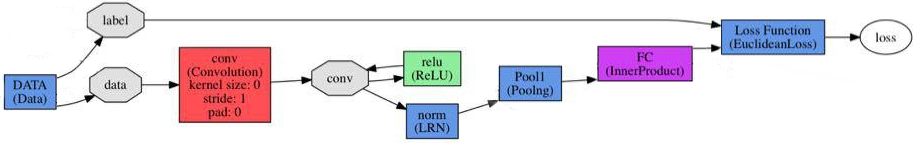
\includegraphics[width=1\textwidth]{images/dcnn}}
	\caption{The basic design for the proposed DCNNs.}
	\label{fig:proposenet}
\end{figure}

The above explanation describes the reasons behind the selected architecture and how it can help us to overcome the deficiencies of previous related works. However, the most important fact regarding DCNNs' capability to learn features is the depth and settings of the architecture which will be attentively addressed later on (chapter~\ref{imparch}).  


\chapter{Implementation}
\label{sec:implementation}
\noindent
In this chapter, we provide a detailed implementation of our proposed methodology. We start by giving insight into the introduced algorithms for generating the synthetic datasets to train and test our models. Then we present the software platform we incorporated to shape and design our architectures. Finally, we demonstrate our networks' architecture and settings in detail. 

%\noindent In this chapter, we provide a detailed implementation of our proposed methodology. We start with presenting the software platform we incorporated to shape and design our models. Then we demonstrate our network's architecture in detail. Finally, we attempt to give insight into the datasets we used to train and test our model. 



\section{The Datasets}
\label{dataha}

Here we delve into the data processing part of this work by introducing three different datasets we created or applied for our empirical experiments. To that end, we provide a detailed explanation for each step of synthetic data generation process along with approaches and methods used to improve each dataset.

%Here we delve into the data processing part of this work by introducing three different datasets we generated or chose for our empirical experiments. To that end, we provide a detailed explanation of the approaches and methods used to generate and improve each dataset.

\subsection{Even-odd Digits Dataset}
\label{subsubsec:digit}

Our Even-odd handwritten dataset contains images of size $100\times100$. Each image is filled with from 0 up to 15 randomly selected digits from MNIST hand-written digits dataset. The process of creating images follows the steps in below:
\begin{enumerate}
\item MNIST Digits are resized to $18\times18$ pixels.
\item Up to 15 digits are randomly put in images of size $100\times100$ pixels.
\item The images are created with controlled overlapping by ensuring that two different numbers are 18 pixels away from each other, i.e. the distance between two digits centers is larger than 18 pixels.
\item Images are labeled with the number of even digits present in each image. 
\item The images are created uniformly, meaning that for example, the number of images containing 0 even digits is equal to the number of images containing 15 even digits.
\end{enumerate}
 This dataset has in total 1 million images: 800,000 images for training set and 200,000 as the test. Figure~\ref{fig:l2cmnist} illustrates some examples of even-odd digits dataset with different number of even digits in images.

\begin{figure}[H]
	\centering
	{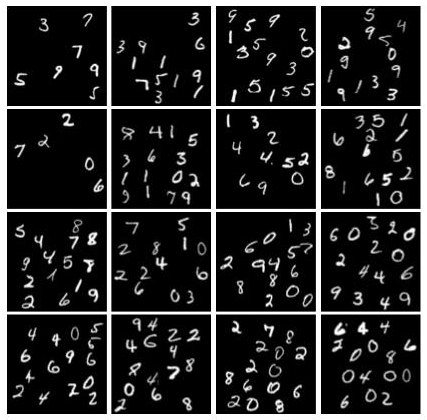
\includegraphics[width=0.5\textwidth]{images/l2cimages}}
		\caption{An example of even-odd digits images. Form left to right, images contain 0 to 15 even digits.}
	\label{fig:l2cmnist}
\end{figure}

%Digits are resized to $18\times18$ pixels and randomly put in the image. The images are created with controlled overlapping by ensuring that two different numbers are 18 pixels away from each other, i.e. the distance between two digits centers is larger than 18 pixels. For the training process, images are labeled with the number of even digits present in each image. Figure~\ref{fig:l2cmnist} illustrates some examples of even-odd digits dataset with different number of even digits in images.

%Our Even-odd handwritten dataset contains images of size $100\times100$. Each image is filled with from 0 up to 15 randomly selected digits from MNIST hand-written digits dataset. Digits are resized to $18\times18$ pixels and randomly put in the image. The images are created with controlled overlapping by ensuring that two different numbers are 18 pixels away from each other, i.e. the distance between two digits centers is larger than 18 pixels. For the training process, images are labeled with the number of even digits present in each image. Figure~\ref{fig:l2cmnist} illustrates some examples of even-odd digits dataset with different number of even digits in images. 

%\begin{figure}[H]
%	\centering
%	{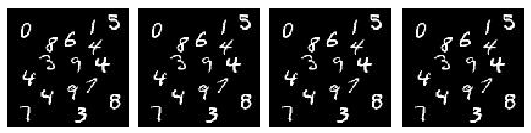
\includegraphics[width=0.9\textwidth]{images/l2cmnist}}
%		\caption{An example of even-odd digits images. Form left to right, images contain 0, 5, 10 and 15 even digits.}
%	\label{fig:l2cmnist}
%\end{figure}

%\indent This dataset has in total 1 million images: 800,000 images for training set and 200,000 as the test. Also, the dataset is uniformly generated, meaning that for instance, the number of images containing 0 even digits is \todo{`the numer' is always `is'} equal to the number of images containing 15 even digits.  

\subsection{Synthetic Pedestrians Dataset}
\label{subsec:synped}

Learning features using deep architectures requires a large amount of data. More importantly, for a fully supervised learning, this data should be annotated. Lack of data or its' high annotation cost prohibit the usage of deep learning methods for many problems including crowd counting. 

\indent However, in order to lower this cost, in our research, we decided to create a synthetic dataset of pedestrians in a walkway. To do that, we used UCSD unlabeled Anomaly detection dataset of pedestrians collected by \citeauthor{chan2008privacy} and used in \cite{chan2009analysis, mahadevan2010anomaly, li2014anomaly}. UCSD Anomaly detection dataset contains clips of groups of people walking towards and away from the camera, and consists of 34 training video samples and 36 testing video samples. Each video has 200 frames of each $238\times158$ pixels. Figure~\ref{fig:anomaly} depicts some images of UCSD Anomaly dataset.

\begin{figure}[H]
	\centering
	{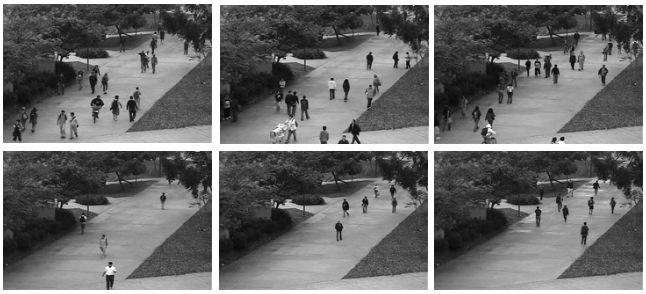
\includegraphics[width=0.7\textwidth]{images/anomaly}}
	\caption{Sample images of UCSD Anomaly detection dataset.}
	\label{fig:anomaly}
\end{figure}


\indent In our study, we used all 70 training and testing video samples to generate the synthetic pedestrians dataset. To thoroughly demonstrate the generation process of our dataset, we divide this section into data generation and data improvement.

  
\subsubsection{Data Generation}

In our dataset, we constrained each image by having up to 29 pedestrians in the walkway. The process of generating the data includes the following steps:
\begin{enumerate}

\item \textbf{Background extraction:} Firstly, we simply subtract the background from each video frame. We extract two types of backgrounds: the median of all the backgrounds in each video (in total, 70 different backgrounds), and the median of all median backgrounds. An example of extracted backgrounds is shown below.

\begin{figure}[H]
	\centering
	{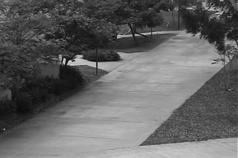
\includegraphics[width=0.4\textwidth]{images/background}}
	\caption{One background image extracted from UCSD dataset.}
	\label{fig:bgim}
\end{figure}


\item \textbf{Pedestrian extraction:} Subtracting each image from the mean background, we were able to label the connected regions (each individual in case of our images) of the subtraction using morphological labeling methods. Figure~\ref{fig:nobg} shows how images look like after background subtraction. 
\begin{figure}[H]
	\centering
	{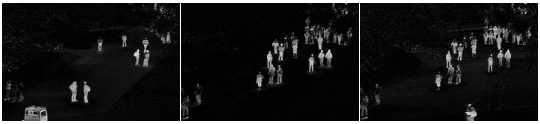
\includegraphics[width=0.9\textwidth]{images/nobg}}
	\caption{Images after background subtraction.}
	\label{fig:nobg}
\end{figure}
 
Then, properties of labeled regions are measured and bound-boxed (see \cite{van2014scikit} for more detailed explanation). Boxes of people are center-based annotated. These labeled boxes shape our initial list of pedestrians with masks of the same size of each box. Figure~\ref{backback} in below demonstrates a selection of extracted pedestrians and pedestrians' masks.

\begin{figure*}[h!]
    \centering
    \begin{subfigure}[t]{0.5\textwidth}
        \centering
        {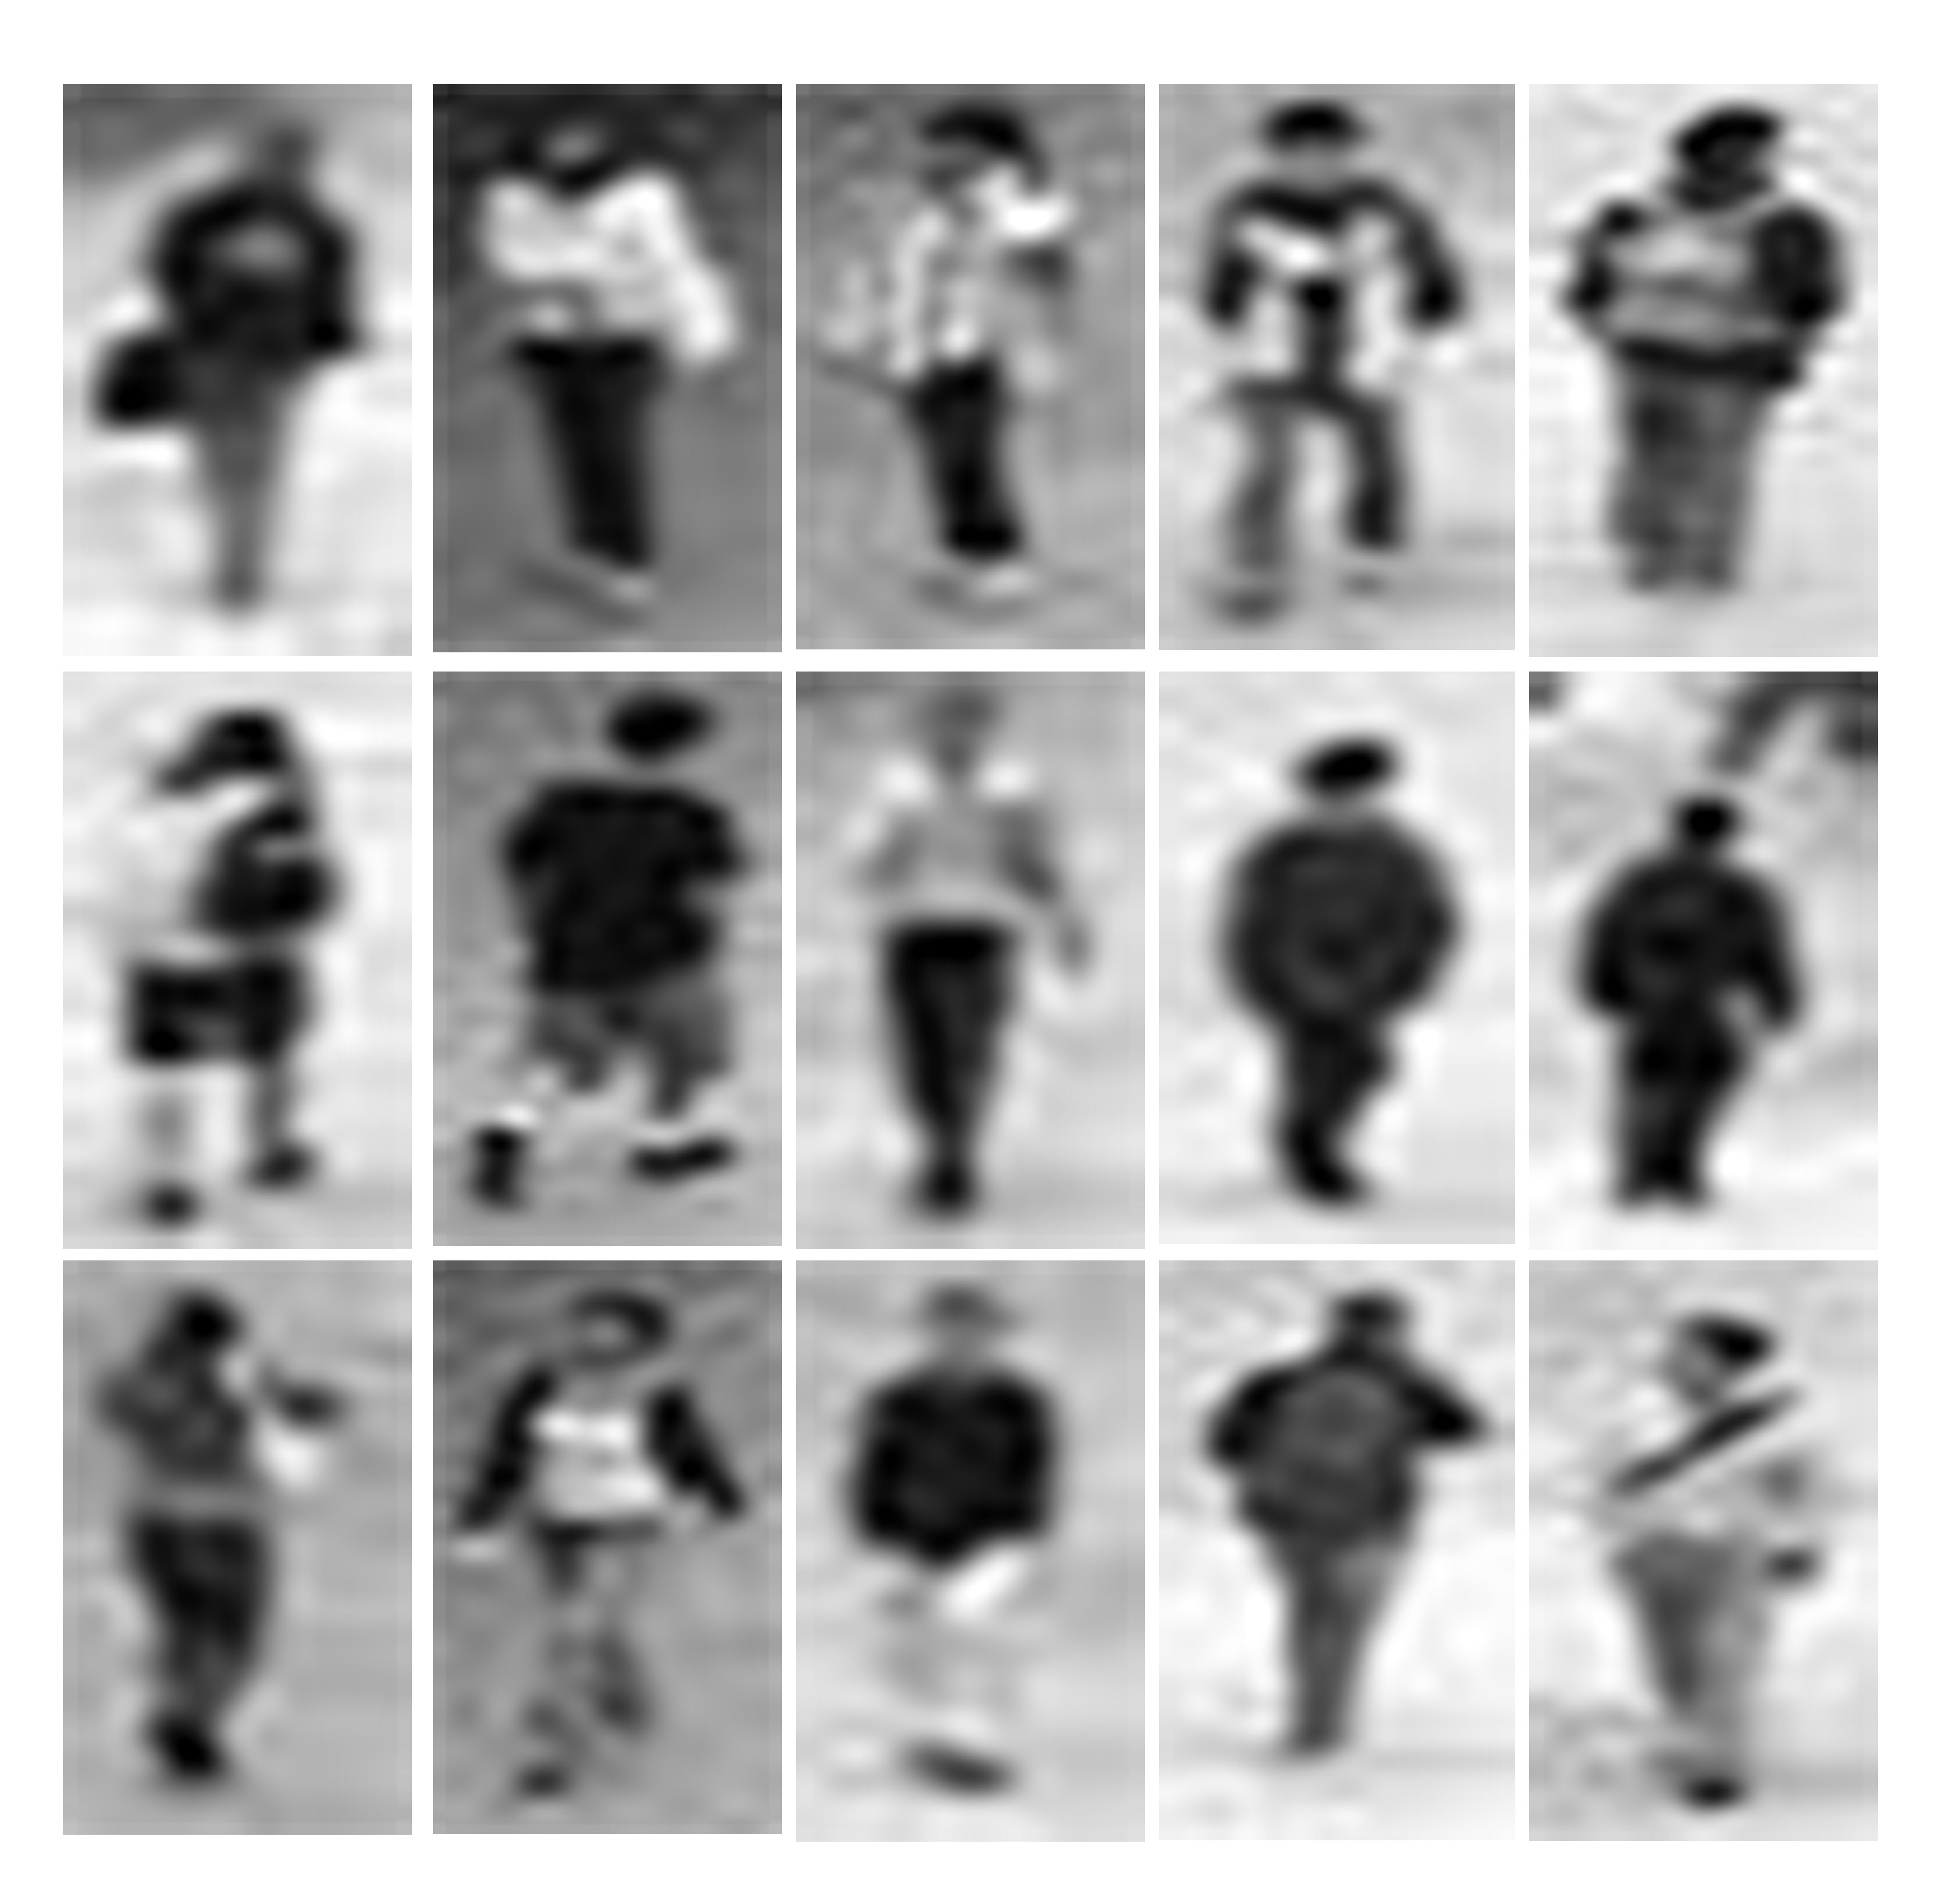
\includegraphics[width=0.5\textwidth]{images/peds}}
        \caption{Extracted pedestrians.}
    \end{subfigure}%
    ~ 
    \begin{subfigure}[t]{0.5\textwidth}
        \centering
        {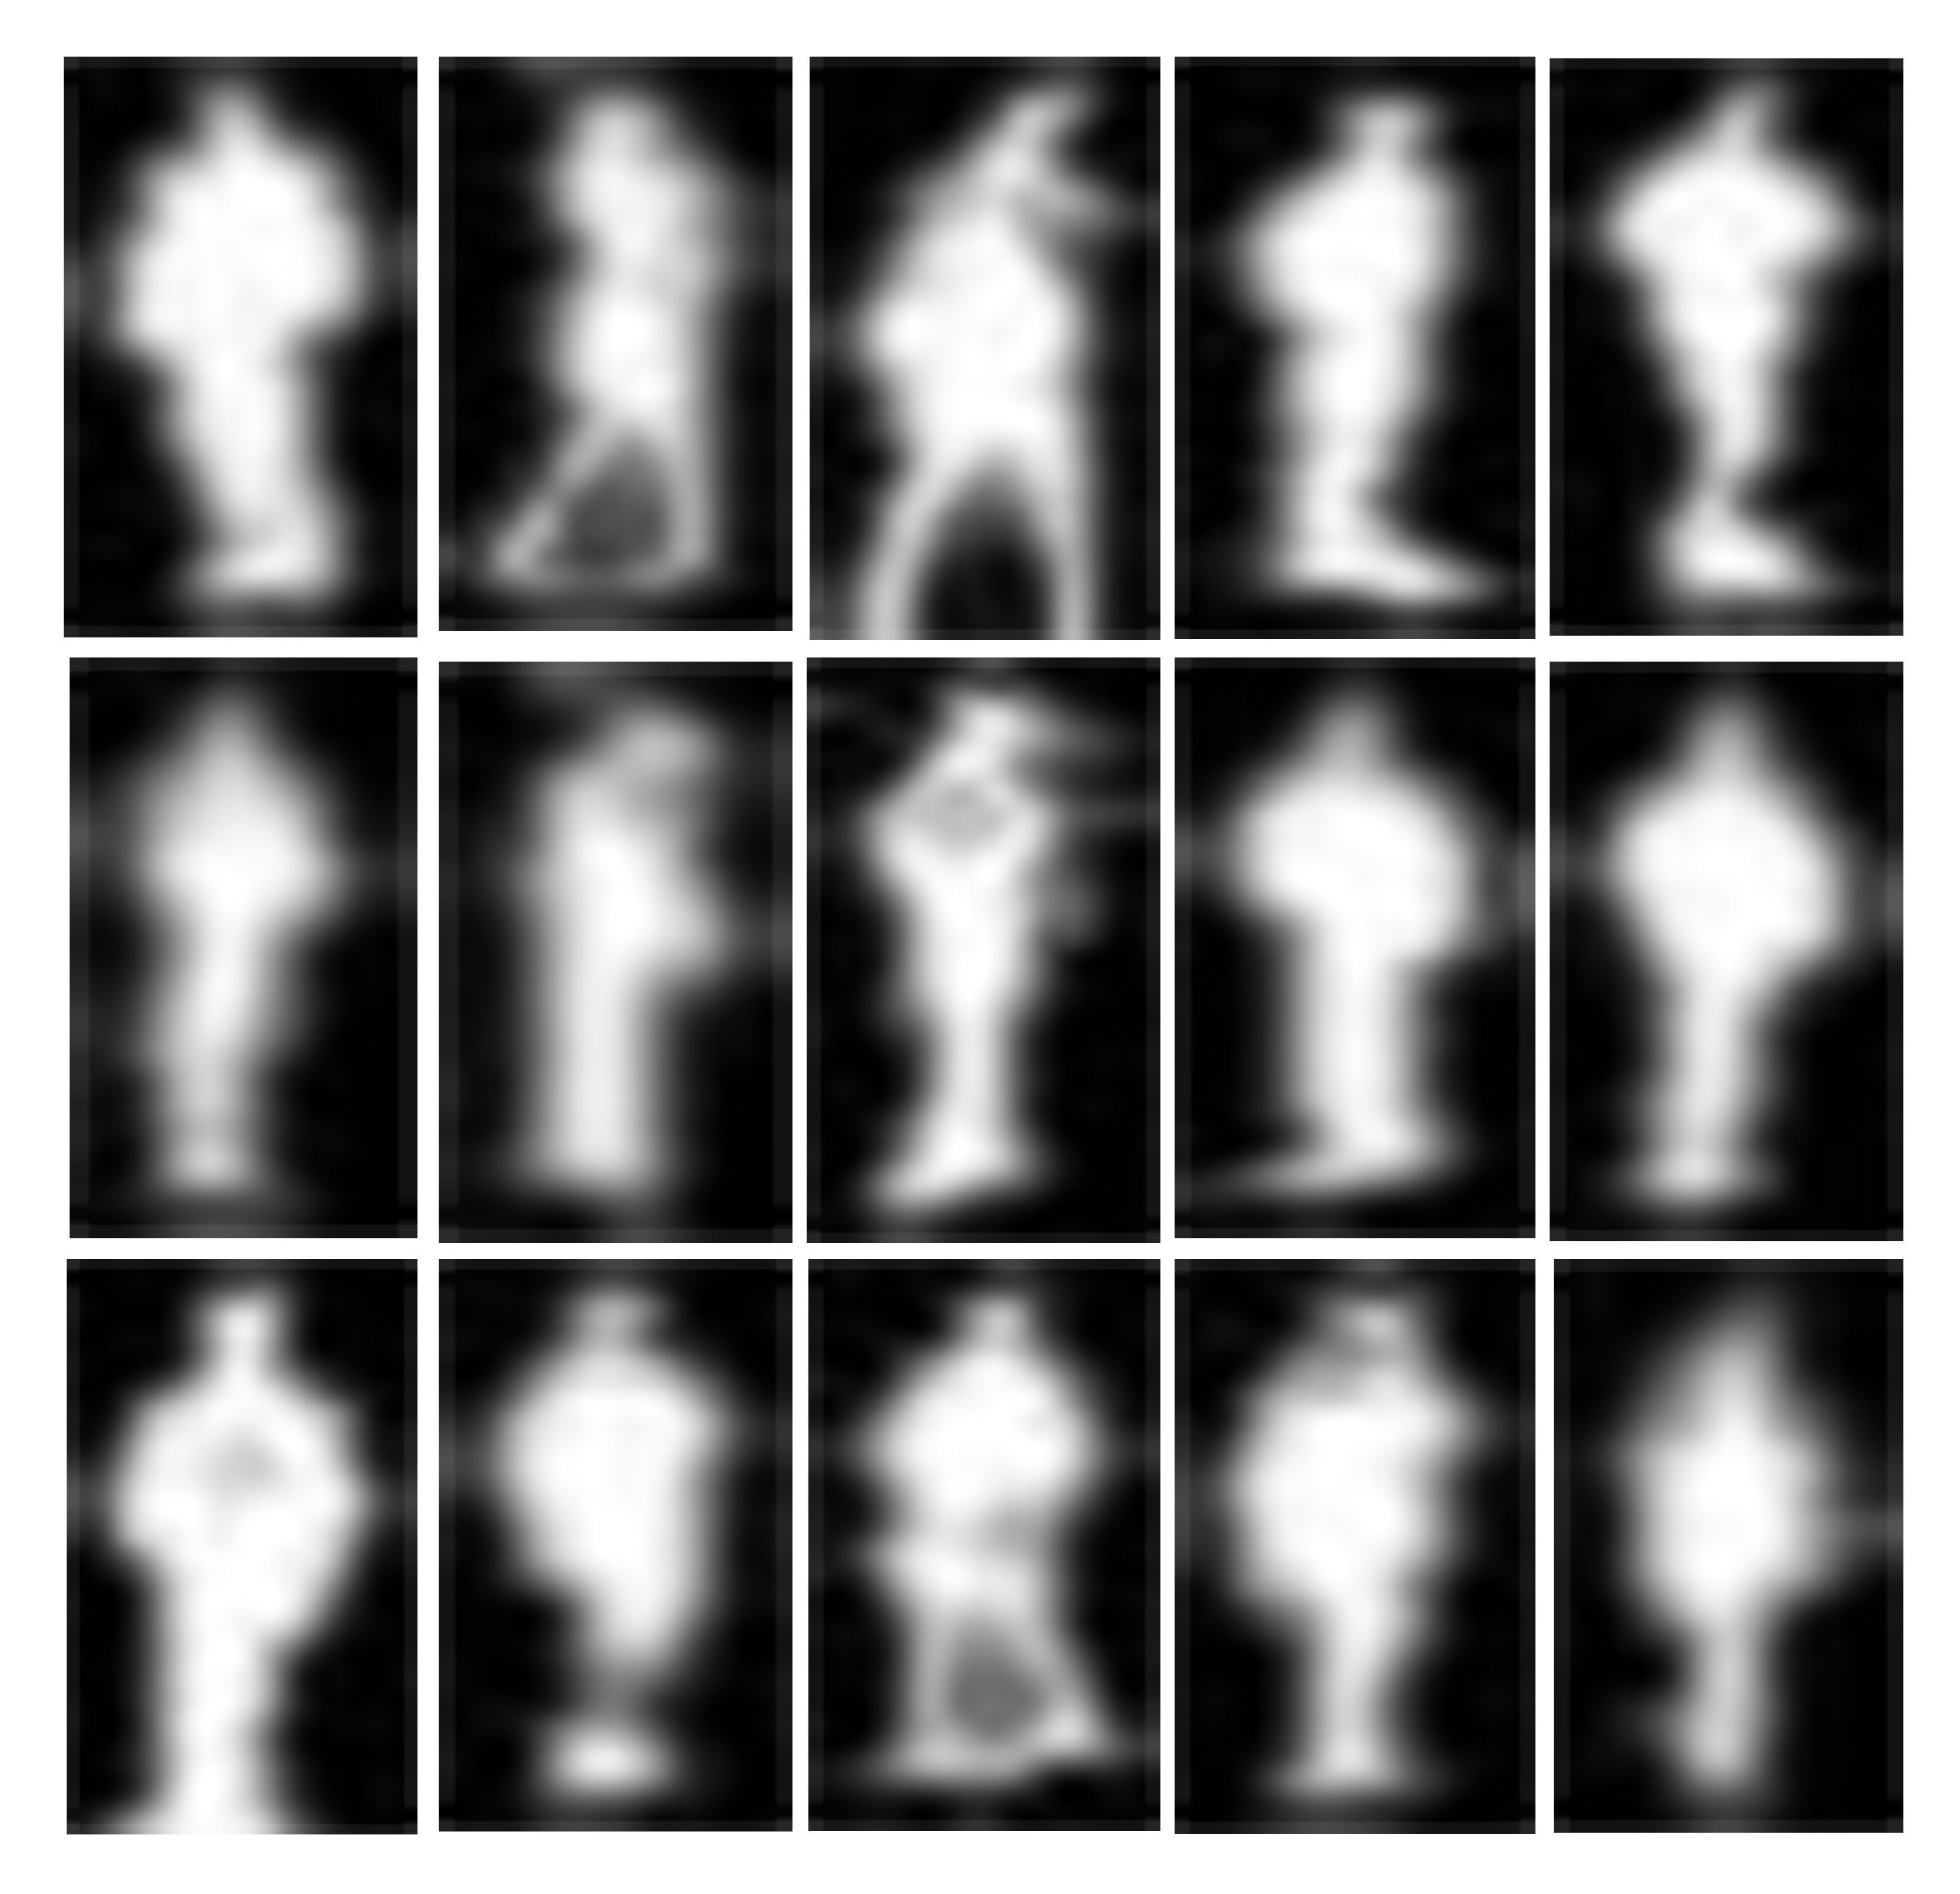
\includegraphics[width=0.5\textwidth]{images/masks}}
        \caption{created pedestrians' masks.}
    \end{subfigure}
    \caption{Pedestrians and their corresponding masks.}
    \label{backback}
\end{figure*}


\item \textbf{Background generation:} In this step, we tried to make the backgrounds of images as realistic as possible by:
\begin{enumerate}
\item making a sparse combination of median backgrounds.
\item changing the global illumination of the images randomly.
\item adding some random Gaussian noise to the backgrounds.
\end{enumerate}
 As you may notice, in the figure~\ref{backback}, the generated background happened to be brighter and noisier than the extracted one.
 
 
%1)~making a sparse combination of median backgrounds, 2)~changing the global illumination of the images randomly, and 3)~adding some \textit{Gaussian noise} to the backgrounds. As you may notice, in the figure~\ref{backback}, the generated background happened to be brighter and noisier than the extracted one. 

\begin{figure*}[h!]
    \centering
    \begin{subfigure}[t]{0.4\textwidth}
        \centering
        {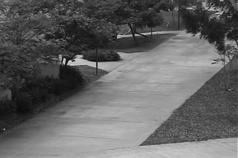
\includegraphics[width=0.8\textwidth]{images/background}}
        \caption{Raw extracted background image.}
    \end{subfigure}%
    ~ 
    \begin{subfigure}[t]{0.4\textwidth}
        \centering
        {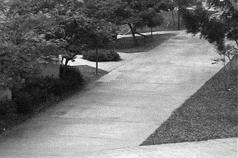
\includegraphics[width=0.8\textwidth]{images/background3}}
        \caption{Generated background after a sparse combination, global illumination change and some noise.}
    \end{subfigure}
    \caption{A synthetically generated background image}
    \label{backback}
\end{figure*}

 Having backgrounds generated and pedestrians extracted and labeled, backgrounds are selected randomly. Then, for training and comparison purposes, images are masked with a filter of \textit{Region Of Interest}~(ROI). The mask and ROI is shown in below (figure~\ref{fig:roi}).

\begin{figure*}[h!]
    \centering
    \begin{subfigure}[t]{0.4\textwidth}
        \centering
        {
\includegraphics[width=0.8\textwidth]{images/catwalk}}
        \caption{ROI mask.}
    \end{subfigure}%
    ~ 
    \begin{subfigure}[t]{0.4\textwidth}
        \centering
        {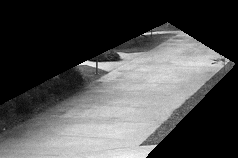
\includegraphics[width=0.8\textwidth]{images/roi}}
        \caption{ROI in the image.}
    \end{subfigure}
    \caption{Applying the mask of region of interest on the background image.}
    \label{fig:roi}
\end{figure*}

\item \textbf{Creating synthetic images:} Afterwards, pedestrians are added to the masked background in a way that the center of each person is placed inside white area of the mask. Finally images are normalized (between 0 and 255) and resized to $158\times158$ in order to be fed to convolution layers. A selection of created images are depicted in the figure underneath.

\begin{figure}[H]
	\centering
	{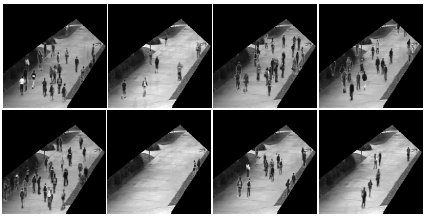
\includegraphics[width=0.8\textwidth]{images/myped}}
	\caption{created synthetic images for counting pedestrians problem.}
	\label{fig:myped}
\end{figure}

\end{enumerate}

\subsubsection{Data Improvement}
\label{dataimp}
Although we managed to successfully create synthetic images of people in the street, the generated images were still quite distinguishable from the real dataset. Thus, in order to make images as highly realistic as possible, we improved the dataset as explained underneath:
\begin{itemize}
\item \textbf{Non-pedestrian objects:} Amongst the extracted boxes of pedestrians, there were some non-pedestrian boxes with objects instead of pedestrians, and yet others with more than one person inside the box. Therefore, we manually removed these outliers. After this edition, we ended with 426 samples of people. A few examples of incorrectly collected or labeled objects are shown in below.

\begin{figure}[H]
	\centering
	{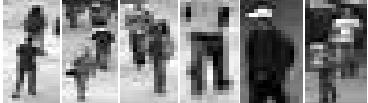
\includegraphics[width=0.6\textwidth]{images/nonped}}
	\caption{A selection of non-human or incorrectly labeled objects. As you may see, there are some images with "half a person" and some others with more than just one person in the image.}
	\label{fig:nonped}
\end{figure}
 
\item \textbf{Lack of pedestrians:} For the sake of generalization, we needed a decent variety of pedestrians in the images to train with. For this purpose, we created 2 versions of current pedestrians list, each darkened by the factor of 20\% from each other. 
\item \textbf{Halos around the pedestrians:} Due to lack of accuracy of the region measuring method, a fine layer of the background that pedestrians were extracted from, still remained around the pedestrians. In the created images, depending on where the person was placed, these thin layers appeared like a halo around the person. Figure~\ref{fig:haloim} illustrates some images with halos around the pedestrians. 
\begin{figure}[H]
	\centering
	{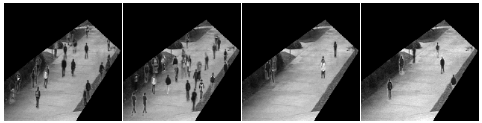
\includegraphics[width=0.8\textwidth]{images/halo}}
	\caption{A few synthetic images with halos around the pedestrians in the walkway.}
	\label{fig:haloim}
\end{figure}
 
To mitigate this issue, we tried two approaches:
\begin{enumerate}
\item \textbf{Morphological erosion:} Among morphological operations on image, we applied \textit{erosion} \cite{van2014scikit} to erode the pedestrians masks. In this way, the halos were ignored to some noticeable extent. 
\item \textbf{Poisson image editing:} Poisson image editing is a technique for seamlessly blending two images together fully automatically  \cite{perez2003poisson}. In addition to erosion, we tried Poisson image editing tool to remove the halos. However, due to our gray-scale and low-resolution images, this tool did not have a great impact on our images.      
\end{enumerate}
Afterwards, the images look similar to the ones shown in figure~\ref{fig:nohalo}.

\begin{figure}[H]
	\centering
	{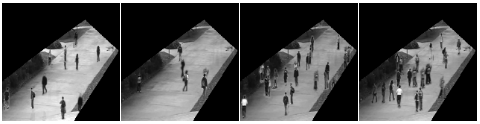
\includegraphics[width=0.8\textwidth]{images/nohalo}}
	\caption{Some examples of images with no or less halo around the people in the images.}
	\label{fig:nohalo}
\end{figure}
 
\item \textbf{Image Perspective:} Since pedestrians of different sizes were put randomly in the images, we considered people's tallness perspective in the images. As you may observe, in the following figure~\ref{fig:nopers}, image perspective has not been applied in the images and hence, there are some pedestrians closer to the camera but really small and also some pedestrians quite tall at the end of walkway.

\begin{figure}[H]
	\centering
	{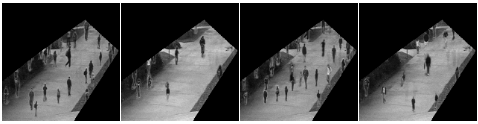
\includegraphics[width=0.8\textwidth]{images/nopers}}
	\caption{created images before considering image perspective.}
	\label{fig:nopers}
\end{figure}

Humans' height almost follows a Gaussian distribution \cite{subramanian2011height}. Therefore, with respect to \cite{subramanian2011height, garcia2007evolution}, we mapped individual's heights with the length of the walkway in the image, considering a Gaussian noise with mean $\mu = 0$ and $\sigma = 3.5$. The resulting images are demonstrated as follows.

\begin{figure}[H]
	\centering
	{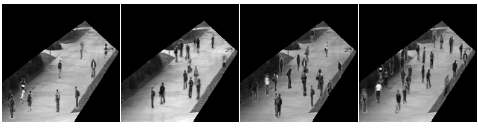
\includegraphics[width=0.8\textwidth]{images/pers}}
	\caption{Synthetic images considering image perspective based on the real distribution of people's height. As you may see, after applying perspective, the images look more realistic. }
	\label{fig:pers}
\end{figure}


\end{itemize}

\noindent Thusly, we created a set of 1 million images, each of size $158\times158$ pixels with up to 29 pedestrians. We assigned 800,000 images for training set and 200,000 instances as the test set. We believe the created synthetic dataset of pedestrians is realistic enough to be able to represent a real-world crowd counting scenario. However, the images can be improved in different aspects and by using diverse image editing and manipulation techniques. 

\subsection{UCSD Crowd counting Dataset}
\label{subsec:datareal2}
To verify and validate our model, we used UCSD crowd counting dataset created by \citeauthor*{chan2008privacy} and used in \cite{chan2008privacy,chan2009bayesian,chan2012counting}. The dataset contains video of pedestrians on UCSD walkways, taken from a stationary camera. There are currently two  viewpoints available among which we used \textit{vidf} videos. All videos are 8-bit gray-scale, each video file has 200 video frames, with dimensions $238\times158$. In our experiment, the first 20 videos which are labeled with the number of pedestrians, were incorporated. The center point of each pedestrian defines its' location in the image. A selection of UCSD crowd counting images is shown in figure~\ref{fig:ucsdorg}.

\begin{figure}[H]
	\centering
	{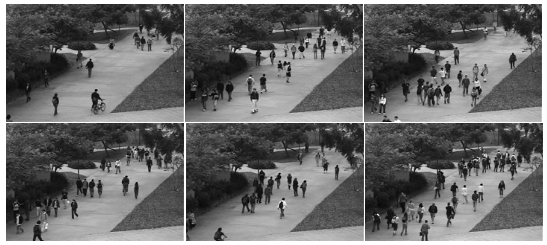
\includegraphics[width=0.8\textwidth]{images/normalucsd}}
	\caption{Normal UCSD crowd counting dataset images.}
	\label{fig:ucsdorg}
\end{figure}

\indent Among the labeled images, we selected the ones in which the number of pedestrians does not exceed 29. Then, images were resized to  $158\times158$ pixels and normalized between 0 and 255. Hence, in total we have a dataset of 3375 real images which are masked with the same filter we used for synthetic pedestrians dataset (shown in figure~\ref{fig:roi}). At last, the images look like the following images.

\begin{figure}[H]
	\centering
	{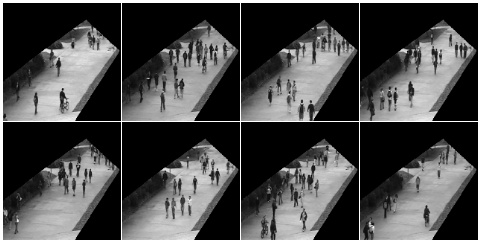
\includegraphics[width=0.8\textwidth]{images/testucsd}}
	\caption{Real UCSD images after being masked and resized.}
	\label{fig:testucsd}
\end{figure}


\indent We will use this dataset to first, validate the performance of our model trained with synthetic data, on a real dataset, and then to do a comparison between the work done in \cite{chan2008privacy} and our approach.



\section{Caffe Deep Learning Platform}

Caffe is a clean and modifiable framework for state-of-the-art deep learning algorithms and a collection of reference models. The framework is a BSD-licensed C++ library with Python and MATLAB bindings for training and deployment of general-purpose convolutional neural networks and other deep models on commodity architectures \cite{jia2014caffe}. It powers on-going research projects and large-scale industrial applications in vision, speech and multimedia by CUDA \footnote{CUDA is a parallel computing platform and application programming interface (API) model created by NVIDIA \cite{cuda}, processing over 40 million images a day on a single K40 or Titan GPU \cite{jia2014caffe}.}  GPU computation.

Caffe is composed of two main components, models' architecture and design, and model optimization. In the rest of this section, we present the main components and parameters of both model implementation and optimization.
\subsection{Model Implementation and Design}
The main components of Caffe architecture are outlined below:
\begin{enumerate}

\item \textbf{Data storage:} Caffe stores and communicates data in 4-dimensional arrays called \textit{blobs}. Blobs provide a unified memory interface, holding batches of data, parameters, or parameter updates. Blobs conceal the computational overhead by synchronizing from the CPU host to the GPU device as needed. Figure~\ref{fig:blob} shows the blobs connected to a convolution layer implemented by Caffe.


\begin{figure}[H]
	\centering
	{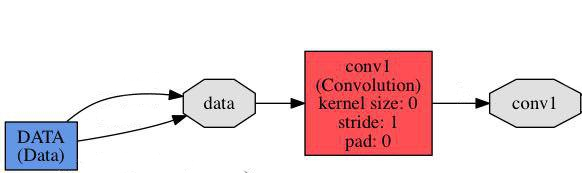
\includegraphics[width=0.7\textwidth]{images/caffeconvlayer}}
	\caption{Input (data) and output (conv1) blobs of a convolution layer in a CNN implemented in Caffe.}
	\label{fig:blob}
\end{figure}


Caffe supports some data sources such as LevelDB or LMDB (Lightning Memory-Mapped Database), HDF5, MemoryData, ImageData, etc. However, large-scale data is stored in LevelDB databases since it reads the data directly from memory \cite{caffe}. 
\item \textbf{Layers:} A caffe layer takes blobs as input and yields one or more as output. In a network (as described in chapter~\ref{subsec:bp}), each layer plays two important roles: a forward pass that takes the inputs and produces the outputs, and a backward pass that takes the gradient with respect to the output, and computes the gradients with respect to the parameters and to the inputs, which are in turn back-propagated to earlier layers \cite{jia2014caffe}.

\indent Caffe supports an exhaustive set of layers, including the followings \cite{jia2014caffe}: 
\begin{enumerate}
	\item Convolution, pooling, fully connected, 
	\item Nonlinearities like rectified
	linear and logistic, local response normalization, element-wise operations, and 
	\item Losses like softmax and hinge
\end{enumerate}
\item \textbf{Networks and run mode:} Caffe ensures the correctness of the forward and backward passes for any directed acyclic graph of layers. A typical network begins with a data layer laying down at the bottom going up to the loss layer that computes tasks' objectives. The network is run on CPU or GPU independent of the model definition. 
\item \textbf{Training a network:} Training phase in Caffe is done by classical stochastic gradient descent algorithm. When training, images and labels pass through different layers lead into the final prediction into a classification layer that produces the loss and gradients which train the whole network. Figure~\ref{fig:caffe} illustrates a typical example of a Caffe network. 


\indent Finetuning, the adaptation of an existing model to new architectures or data, is a standard method in Caffe. Caffe  finetunes the old model weights for the new task and initializes new weights as needed. This capability is essential for tasks such as knowledge transfer \cite{donahue2013decaf}, object detection \cite{girshick2014rich}, and object retrieval \cite{guadarrama2014open}, \cite{jia2014caffe}.  
\end{enumerate}


\begin{figure}[H]
	\centering
	{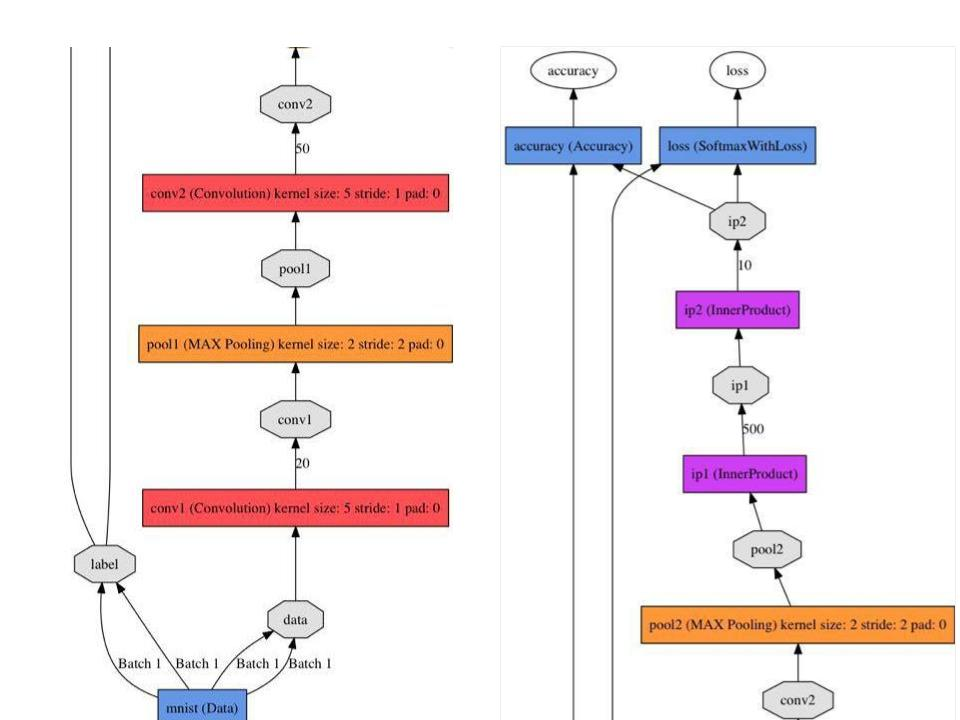
\includegraphics[width=0.9\textwidth]{images/le2col}}
	\caption{From bottom-left to top-right, Lenet architecture for MNIST digit classification example of a Caffe network, where boxes represent layers and octagons represent data blobs produced by or fed into the layers \cite{jia2014caffe}.}
	\label{fig:caffe}
\end{figure}

\textbf{Justification}: We decided to use Caffe because, it addresses computation efficiency problems (as likely the fastest available implementation of deep learning frameworks at the time of performing this study, adheres to software engineering best practices, providing unit tests for correctness and experimental rigor and speed for deployment. It is also well-suited for research use, due to the well-implemented modularity of the code, and the clean separation of network definition (usually the novel part of deep learning research) from actual implementation\cite{jia2014caffe}. In addition, it provides a python wrapper which exposes the solver module for easy prototyping of new training procedures. 

\subsection{Model Optimization}

Our work in general is an optimization problem since we project the results as loss functions we try to minimize. For this reason, model optimization methods have a critical impact on the performance of the model. In Caffe, \textit{Solver} file orchestrates optimization by coordinating the network's forward inference and backward gradients to form parameter updates that attempt to improve the loss. Among Caffe solver methods, we use stochastic gradient descent (explained in chapter~\ref{subsec:sgd}). The use of SGD in deep convolutional neural network setting is motivated by the high cost of running back propagation over the full training set. SGD can overcome this cost and still lead to fast convergence. 

Although Caffe provides several optimization methods, in this section we briefly describe merely optimization methods and \textit{hyper-parameters}\footnote{Hyper-parameters govern the underlying system on a "higher level" than the primary parameters of interest. They are not model parameters that are learned during training phase and instead, they are set by the designer a priori.} incorporated in our proposed algorithms.


\subsubsection{Batch Size}

Since Caffe is trained using stochastic gradient descent, at each iteration, it computes the (stochastic) gradient of the parameters with respect to the training data and updates the parameters in the direction of the gradient. On the other hand, to compute the gradient w.r.t the input data, we need to evaluate all training samples at each iteration which is prohibitively time-consuming, specially when we are dealing with a great amount of data. 

\indent In order to overcome this issue, SGD approximates the exact gradient, in a stochastic manner, by sampling only a small portion of the training data at each iteration. This small portion is the \textit{batch}. In other words, the batch size defines the amount of training data we feed to the network at each iteration. The larger the batch size, the more accurate the gradient estimate at each iteration will be. 

\subsubsection{Learning Rate}
\label{learning rate}
Learning rate is a decreasing function of time. It's a common practice to decrease the base learning rate (base\_lr) as the optimization/learning process progresses. In Caffe, different learning policies exist among which we tried the followings:
\begin{itemize}
\item \textit{\textbf{Fixed}:} which always returns the base learning rate.

\item \textit{\textbf{inv}:} which returns $$base\_lr \times (1 + \gamma \times iteration) ^ {(-Power)}$$ where:\\\textit{ $\gamma$: the factor learning rate drops by.}\\\textit{power: another parameter to compute the learning rate.}

\item \textit{\textbf{step}:} that returns $$base\_lr \times \gamma ^ {floor(\frac{iteration}{step})}$$ where:\\ \textit{$\gamma$: the factor learning rate drops by.}\\\textit{step: the number of iteration at which the learning rate drops.} 
\item \textit{\textbf{multi-step}:} similar to step but it allows non uniform steps defined by step value.
\end{itemize}
Although there are numerous empirical studies and rules of thumb to treat learning rate \cite{senior2013empirical,yu1995dynamic,minai1990acceleration}, basic learning rate and learning policy are highly problem-dependent.  

\subsubsection{Weight Decay}


As a part of Back Propagation and a subset of regularization methods, \textit{weight decay} adds a penalty term to the error function by multiplying weights to a factor slightly less than 1 after each update. 

 It has been observed in numerical simulations that a weight decay can improve generalization in a feed-forward neural network. It is proven that weight decay has two effects in a linear network. Firstly, it suppresses any irrelevant components of the weight vector by choosing the smallest vector that solves the learning problem. Secondly, if the size is chosen correctly, a weight decay can suppress some of the effects of static noise on the targets, which improves generalization significantly \cite{moody1995simple}. 

\subsubsection{Momentum}
%\todo{doesn't it belong to state-of-the art / implementation??cant put it in implementation cuz its built-in caffe and I just set the value. Hence, I thought they are better off here since they belong also to model optimization?}
One of the potential problems with stochastic gradient descent is having oscillations in the gradient, since not all examples are used for each calculation of the derivatives. This can cause slow convergence of the network. One strategy to mitigate this problem is the use of \textit{Momentum}. The momentum method introduced by \citeauthor{polyak1964some}, \citeyear{polyak1964some}, is a first-order optimization method for accelerating gradient descent that accumulates a velocity vector in directions of persistent reduction in the objective across iterations. Given an objective function $f(\theta)$ to be minimized, momentum is given by:
\begin{equation}
	\label{eq:t}
	\begin{aligned}
		\nu_{t+1} = \mu\nu_t - \alpha\nabla 
	\end{aligned}
\end{equation}
\begin{equation}
	\label{eq:t}
	\begin{gathered}
	\theta_{t+1} = \theta_t + \nu_{t + 1}
	\end{gathered}
\end{equation}
where $\alpha > 0$ is the learning rate, $\mu \in [0,1]$ is the momentum coefficient, and $\nabla f(\theta_t)$ is the gradient at $\theta_t$ \cite{sutskever2013importance}. 

For example, if the objective has a form of a long shallow ravine leading to the optimum and steep walls on the sides, standard SGD will tend to oscillate across the narrow ravine since the negative gradient will point down one of the steep sides rather than along the ravine towards the optimum \cite{sgd}. The objectives of deep architectures have this form near local optima and thus standard SGD can lead to very slow convergence particularly after the initial steep gains. 

Momentum, by taking the running average of the derivatives, by incorporating the previous update in the update for the current iteration, is one method for pushing the objective more quickly along the shallow ravine \cite{sgd}. 

\subsubsection{Number of Iterations}

In learning process, common convergence criteria are: a maximum number of iteration; a desired value for the cost function is reached; or training until the cost function shows no improvement in a number of iterations. In our implementation, we use the maximum number of iteration as our systems' convergence policy. 
 
The number of iterations plays an important role in the training process. iteration number is in an inverse correlation with the number of instances and also the batch size. In any network, batch size and iteration number compensate for one another. For instance, in case of lack of memory, one option would be to decrease the batch size and increase the number of iterations accordingly.


\section{The Architecture}
\label{imparch}

Having Caffe platform introduced, we propose two CNN-based deep architectures for the analysis we did regarding two learning to count problems, counting the number of even-digits and the number of pedestrians in an image.  
In learning object features for vision tasks and by the use of DCNN, the depth of network plays a crucial role. The deeper the model, the better it learns. However, issues like overfitting\footnote{Overfitting occurs when a statistical model describes random error or noise instead of the underlying relationship, and vice versa for underfitting. } and underfitting should not be left neglected.   
Therefore, in this section, networks' settings and architectures for even-digits and crowd counting problems will be described separately. 

\subsection{Even-digit Counting}
\label{subsubsec:digitarch}

For learning to count even digits problem, since we used MNIST dataset to generate our images, we considered the architecture proposed by \citeauthor{lecun1995comparison} for classic MNIST hand-written digit recognition problem \cite{lecun1995comparison} (shown in figure~\ref{fig:caffe}), as the base of our design. In addition, we took into account the architecture used in state-of-the-art \cite{segui2015learning}. Figure~\ref{santil2cfull} demonstrates this architecture. From there, we modified the architecture to optimize the performance of the network. 
 
\begin{figure}[H]
  \centering
   {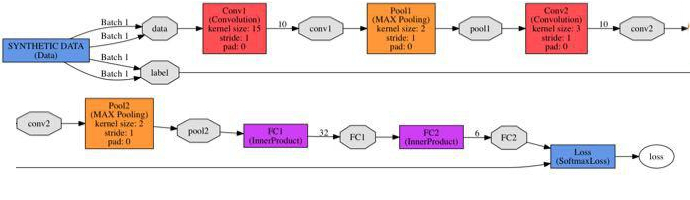
\includegraphics[width=1.\textwidth]{images/santil2cfull}}
  %\end{center}
	\caption{From top-left to bottom-right, the network proposed in \cite{segui2015learning} for Even digits recognition task.}
	\label{santil2cfull}
\end{figure}

\noindent In a similar experiment with maximum 5 digits in images, \citeauthor{segui2015learning} in \cite{segui2015learning} defined a four layers CNN with two convolutional layers for classifying even digits present in images. Each convolutional layer consists of several elements: a set of convolutional filters, ReLU non-linearities, max pooling layers and normalization layers. The first convolutional layer outputs 10 filters of dimensions $15\times15$, and the second convolution layer has 10 filters, each of size $3\times3$. Each convolution layer is followed by a max-pooling layer with a $2\times2$ kernel. The output of last pooling layer is fed to two fully-connected layers with respectively 32 and 6 number of outputs. They also used Softmax loss layer on top of their architecture to compute the multinomial logistic loss layer\footnote{This function displays a similar convergence rate to the hinge loss function, and since it is continuous, gradient descent methods can be utilized. Also, functions which correctly classify points with high confidence are penalized less. This structure is highly sensitive to outliers in the data.}. Table~\ref{santil2c} presents the main components of the network designed by \cite{segui2015learning}. 

\begin{table}[H]
	\centering
	\begin{tabular}{ |p{2cm}|p{2cm}| }
	\hline 
	\multicolumn{2}{|c|}{\textbf{Network parameters}} \\
	\hline
	\hline
	\textbf{Layers} & \textbf{setting }\\
	\hline
	Conv1 & $10\times15\times15$\\
	\hline
	Pool1    & $max(2\times2)$ \\
	\hline
	Conv2 & $10\times3\times3$\\
	\hline
	Pool2 &    $max(2\times2)$ \\
	\hline
	FC1 & 32 outputs \\
	\hline
	FC2 & 6 outputs \\
	\hline
	\end{tabular}
		\caption{The DCNN proposed by \cite{segui2015learning} for learning the number of even digits present in the images.}
		\label{santil2c}
\end{table}
 

\noindent However, in our implementation, due to higher complexity, we decided to apply a deeper CNN with more parameters. In our network, the data layer fetches the images and labels from the disk, passes it through the first convolutional layer with 20 filters, each of size $15\times15$ followed by a ReLU non-linearity and LRN normalization layer. Then the output is max-pooled by the  kernel size of $2\times2$. This process repeats again but this time with the second convolutional layer having 50 filters of size $3\times3$. In all convolution and pooling layers, the \textit{stride} = 1 and \textit{padding}\footnote{Zero padding is a simple concept; it simply refers to adding zeros to end of an image to increase its length.} = 1 are considered (see section~\ref{convlayer} for more explanation regarding padding and stride). 

\noindent the output of the second pooling layer is fed to two fully connected (inner product) layers with respectively 64 and 1 number of outputs (since the problem is approached as a regression task). Also the first fully connected layer is followed by ReLU non-linearity. 


However, a well-designed network cannot solely guarantee an optimal performance for the model. The responsibilities of learning are divided between the network for yielding loss and gradients, and the optimization methods (solver) and parameters for overseeing the optimization and generating parameter updates. Among Caffe solvers, As described in section~\ref{subsec:sgd}, we use Stochastic Gradient Descent optimization method. Apart from solver method, the solver parameters (network's hyper-parameters) need to be set attentively in order to optimize the model performance. Therefore, to optimize the model performance, the networks' hyper-parameters are set as below while table~\ref{hypers} provides a summary of the hyper-parameters' settings. 
\begin{itemize}

\item \textbf{Batch size:} Due to the non-complex and low-resolution dataset we are training on, we were able to use batches of size 256 for our training and testing phases.

\item \textbf{Learning rate:} After trying different initial values in range of $(10^{-6}, 1)$, we set the basic learning rate to $\alpha = 0.0001$. However, for our experiment we chose \textit{multi-step} learning policy in which, after each \textit{stepsize}=40000 iterations, the learning rate drops by the rate of Gamma $\gamma = 0.1$. This initialization is based on rules of thumb used in \cite{krizhevsky2012imagenet}.

\item \textbf{Momentum:} We use momentum $\mu = 0.9$. Because, momentum setting $\mu$ effectively multiplies the size of our updates by a factor of $\frac{1}{1-\mu}$. Hence, changes in momentum and learning rate ought to be accompanied with an inverse correlation. When momentum $\mu = 0.9$, we have an effective update size of 10 since we also drop the learning rate by the factor of $\gamma= 0.1$.

%
%\item \textbf{Momentum:} We use momentum $\mu = 0.9$. This selection also is based on trial and error. As momentum value $\mu$ effectively multiplies the size of our updates by a factor of $\frac{1}{1-\mu}$. Hence, changes in momentum and learning rate ought to be accompanied with an inverse correlation. When momentum $\mu = 0.9$, we have an effective update size of 10 since we also drop the learning rate by the factor of Gamma $\gamma= 0.1$.

\item \textbf{Weight decay:} Weight decay as a penalty term to the error function, has a constant value of 0.0005. This decay constant is multiplied to the sum of squared weights.

\item \textbf{Iterations:} Given the time and hardware we had, we managed to let the system train for 1,600,000 iterations.

\end{itemize}

\begin{table}[H]
	\centering
	\begin{tabular}{ |p{3.8cm}|p{1.7cm}| }
	\hline 
	\multicolumn{2}{|c|}{\textbf{Network hyper-parameters}} \\
	\hline
	\hline
	\textbf{Hyper-parameters} & \textbf{setting }\\
	\hline
	Learning rate & 0.0001\\
	\hline
	Learning policy    & \textit{Multi\_step} \\
	\hline
	Momentum & $\mu = 0.9$\\
	\hline
	Weight decay & 0.0005 \\
	\hline
	Batch size & 256 \\
	\hline
	Iterations & 1600000 \\
	\hline
	\end{tabular}
		\caption{Proposed settings for network's hyper-parameters for counting number of even digits task.}
		\label{hypers}
\end{table}
 

\noindent We should also mention that at the top layer of the network, we used Euclidean Loss layer to compute the euclidean distance between the predictions and the ground truth.  Figure~\ref{fig:l2cNet} shows a scheme of the architecture.
\begin{figure}[H]
  \centering
   {
\includegraphics[width=0.7\textwidth]{images/1}}
  %\end{center}
	\caption{Proposed network architecture for Even digits counting task}
	\label{fig:l2cNet}
\end{figure}

%\todo{this is a useless statement, unless you go into detail what heuristics you've used. justification needed for your choise. so beef it up here between these two sentences}
The architecture has been designed intuitively and based on a heuristic approach where we tried different values for each hyper-parameter at a time and selected the values that provided us with an improvement in the performance of the network. Hence, one may be able to improve the performance by implementing a different architecture or with another settings for the hyper-parameters of the network. 

\subsection{Crowd Counting}
\label{subsec:ucsdarch}

For the task of counting pedestrians, due to the more complex images than the previous task, we designed a deeper architecture. Moreover, we applied the same settings of hyper-parameters to a different architecture. However, as a reminder, table~\ref{hypar2} summarizes the network's settings for the hyper-parameters.

\begin{table}[H]
	\centering
	\begin{tabular}{ |p{3.8cm}|p{1.7cm}| }
	\hline 
	\multicolumn{2}{|c|}{\textbf{Network hyper-parameters}} \\
	\hline
	\hline
	\textbf{Hyper-parameters} & \textbf{setting }\\
	\hline
	Learning rate & 0.0001\\
	\hline
	Learning policy    & \textit{Multi\_step} \\
	\hline
	Momentum & $\mu = 0.9$\\
	\hline
	Weight decay & 0.0005 \\
	\hline
	Batch size & 256 \\
	\hline
	Iterations & 1600000 \\
	\hline
	\end{tabular}
		\caption{Proposed settings for network's hyper-parameters for counting pedestrians.}
		\label{hypar2}
\end{table} 

As a baseline, we considered state-of-the-art architecture designed by \citealt*{segui2015learning} for counting the number of pedestrians in the images. As shown in figure~\ref{santiucsdnet}, in their work, they used a five layer architecture CNN with two convolutional layers followed by three fully connected layers. Convolutional layers contain their main elements (ReLU and LRN layers), and each outputs 8 filters with kernel sizes $9\times9$ and $5\times5$ respectively. 

\begin{figure}[H]
  \centering
   {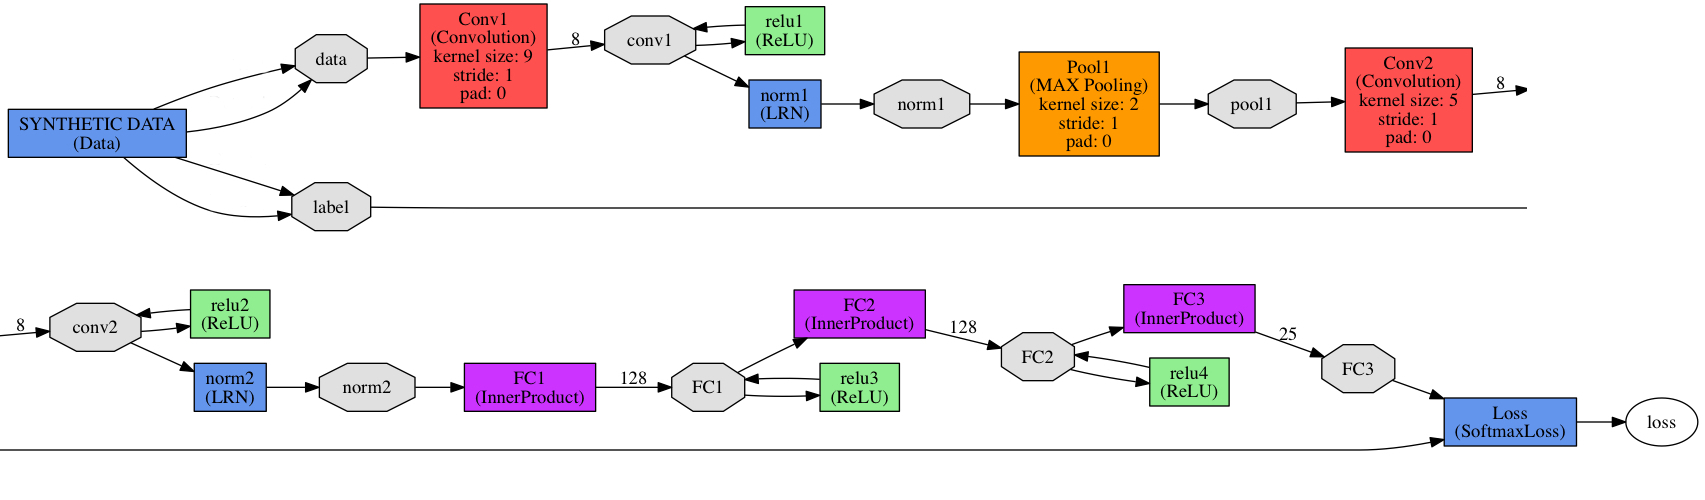
\includegraphics[width=1.00\textwidth]{images/santiucsd}}
  %\end{center}
	\caption{From top-left to bottom-right, the DCNN proposed by \cite{segui2015learning} for learning to count the number of pedestrians in a walkway.}
	\label{santiucsdnet}
\end{figure}

They applied only one max-pooling layer and after the first convolutional layer in their design. Finally, three fully connected layers with number of outputs 128, 128 and 25 classify the output of the network into 25 classes (maximum pedestrians in the images) of the number of people in the image. Similar to the previous task, a softmax loss layer projects the performance of the model.   
Table~\ref{santiarch} describes a summary of their network.

\begin{table}[H]
	\centering
	\begin{tabular}{ |p{2cm}|p{2cm}| }
	\hline 
	\multicolumn{2}{|c|}{\textbf{Network parameters}} \\
	\hline
	\hline
	\textbf{Layers} & \textbf{setting }\\
	\hline
	Conv1 & $8\times9\times9$\\
	\hline
	Pool1    & $max(2\times2)$ \\
	\hline
	Conv2 & $8\times5\times5$\\
	\hline
	FC1 & 128 outputs \\
	\hline
	FC2 & 128 outputs \\
	\hline
	FC3 & 25 outputs \\
	\hline
	\end{tabular}
		\caption{The deep CNN proposed by \citealt{segui2015learning} for learning the number of pedestrians in a walkway.}
		\label{santiarch}
\end{table}


\noindent However, since up to 29 pedestrians are present in our images with high amount of overlapping, in our design we added one convolutional layer to the base architecture. We also increased the number of parameters in the network. In our architecture, the data blobs pass through 4 convolutional layers. The first convolutional layer has 4 filters, each with $5\times5$ kernel and the other 3 layers have again 4 filters but each of size $3\times3$. Similar to the previous model, each convolutional layer is followed by ReLU non-linearity layer and LRN normalization layer. Also the stride and padding values for all the convolutional layers are respectively equal to 1 and 0. 
%\todo{ok, i really want a figure showing the architecture of the network you've designed. it should show the layers, kernels, ... a zoom-in, no full-scale representation needed, just a cutout}

\indent In order to not lose information, we used merely two pooling layers for the first two convolutional layers. Each pooling layer has a kernel size of $2\times2$ with $stride = 1$  and $padding = 0$. Figure~\ref{fig:ucsdnet} illustrates the proposed architecture. 

\begin{figure}[H]
  \centering
   {
\includegraphics[width=0.7\textwidth]{images/1}}
  %\end{center}
	\caption{Proposed network architecture for learning the number of pedestrians in the image.}
	\label{fig:ucsdnet}
\end{figure}

As you may see in figure~\ref{fig:ucsdnet} above, there are three fully connected layers to regress the number of pedestrians in images. The first two fully connected layers have 16 outputs each, and are connected to ReLU non-linearity layers. The last layer however, with solely one output, passes the models' prediction of the number of pedestrians to the Euclidean loss layer to calculate the sum of squares of differences of its two inputs, the true labels and predictions. 
%In figure~\ref{fig:ucsdnet}, an illustration of this architecture has been presented.

To the best of our knowledge, the designed architectures outperform other architectures we tried previously (a different range of architectures starting from 1 up to 5 convolutional layers with different settings), while also fastening the training phase . However, apart from the basic knowledge about network architectures, hyper-parameters initialization and some rules of thumb of successful experiences in similar works, the rest of design has been done intuitively. Therefore, similar to the first architecture (problem of counting even digits), there would be other ways to improve the architecture and performance of the model.




\newpage
\chapter{Experiments and results}
\label{sec:experiments}

Prior to jumping to the final results obtained with our algorithm, this
chapter will attempt to give insight into the experiments we designed to verify our hypothesis. We examine our proposed methodology on two different but related scenarios. In the former scenario, we tackle the learning to count even hand-written digits, for the latter one, crowd counting problem is considered.   
This chapter contains experiments details, obtained results, comparison to similar works and finally a conclusion about the performance of our models in each of the experiments.

\section{Learning to count Even-odd hand-written digits}

We intend to explore the features learned when training a deep CNN, in order to understand their underlying representations. To this end, we designed a synthetic problem of counting even digits in images. This experiment clearly illustrates the basic idea behind this work, where we hypothesize that the features learned during this task are:
\begin{enumerate}
\item Efficient descriptors of digits to enable the model to count them.
\item Sufficiently representative of the digits to be applied for digits recognition tasks. 
\end{enumerate}

In this experiment, we feed images of digits into a deep convolutional neural network. Images are labeled with the number of even digits in each image. We apply a regression strategy to tackle this problem. Therefore, the output of the network is a single number determining the model's prediction for the amount of even digits present in the images. 
 

\subsection{Dataset} 
As it was meticulously described in (section ~\ref{subsubsec:digit}), we synthetically generated \textit{Even-odd digits dataset} to use for this task. the dataset holds the following properties:
\begin{itemize}
\item Images of MNIST hand-written digits where each image contains up to 15 digits. Also the images are made in gray-scale.
\item Each image has a dimension of $100\times100$. And each digit in the image is $18\times18$ pixels.  
\item A minimum distance of 18 pixels is considered between each two digits (from center to center) in an image to prevent overlapping.
\item The dataset is generated uniformly. It means that there are equal number of images for each amount of digits in the image. For instance, the number of images with 5 even digits are the same as number of images containing 10 even digits.
\item The dataset of 1,000,000 samples is divided into a training set of 800,000 and a test set of 200,000. 
\end{itemize}

Since we use Caffe platform to do our experiments, we convert the images into LMDB format. LMDB uses memory-mapped files, so it has the read performance of a pure in-memory database while still offering the persistence of standard disk-based databases, and is only limited to the size of the virtual address space, (it is not limited to the size of physical RAM). Therefore, we created two LMDB files for training and testing sets to be fed to the network.  

\subsection{Learning process}

As discussed in chapter~\ref{subsubsec:digitarch}, for learning to count the number of even digits, we designed a deep CNN. Table~\ref{fig:digitnet} shows a review of the network's specification and architecture.

\begin{table}[H]
	\centering
			\caption{The deep CNN with 2 convolution layers to count the number of even digits.}
	\begin{tabular}{ |p{2cm}|p{2cm}| }
	\hline 
	\multicolumn{2}{|c|}{\textbf{Network parameters}} \\
	\hline
	\hline
	\textbf{Layers} & \textbf{setting }\\
	\hline
	Conv1 & $20\times15\times15$\\
	\hline
	ReLU1 & max(x,0)  \\
	\hline
	LRN1 & $\alpha$=0.0001, $\beta$=0.75\\
	\hline
	Pool1    & $max(2\times2)$ \\
	\hline
	Conv2 & $50\times3\times3$\\
	\hline
	ReLU2 & max(x,0)  \\
	\hline
	LRN2 & $\alpha$=0.0001, $\beta$=0.75\\
	\hline
	Pool2    & $max(2\times2)$ \\
	\hline
	IP1 & 64 outputs \\
	\hline
	ReLU3 & max(x,0)  \\
	\hline
	IP2 & 1 outputs \\
	\hline
	\end{tabular}
		\label{fig:digitnet}
\end{table}




However, a well-designed network solely cannot guarantee an optimal performance for the model. The responsibilities of learning are divided between the Net for yielding loss and gradients, and the optimization methods and parameters for overseeing the optimization and generating parameter updates. 

Among Caffe solvers, As described in section~\ref{subsec:sgd}, we use Stochastic Gradient Descent optimization method. Apart from solver method, we solver parameters need to be set attentively in order to optimize the model performance. Table~\ref{tab:digitsolver} summarizes the initial settings for the solver parameters while the upcoming items justify our decisions.

\begin{table}[H]
	\centering
			\caption{The solver parameters settings for even digit counting problem.}
	\begin{tabular}{ |p{2cm}|p{2cm}| }
	\hline 
	\multicolumn{2}{|c|}{\textbf{Optimization parameters}} \\
	\hline
	\hline
	\textbf{Parameter} & \textbf{value}\\
	\hline
	base\_lr & 0.0001\\
	\hline
	batch size & 256\\
	\hline
	momentum & 0.9  \\
	\hline
	weight decay & 0.0005\\
	\hline
	step size   & 40000 \\
	\hline
	gamma($\gamma$) & 0.1\\
	\hline
	iterations & 1,600,000\\
	\hline
	\end{tabular}

		\label{tab:digitsolver}
\end{table}


\begin{itemize}
\item \textbf{Learning rate:} The basic learning rate is 0.0001. However, for our experiment we chose \textit{multi-step} learning policy in which, after each \textit{stepsize}=40000 iterations, the learning rate drops by the rate of $\gamma = 0.1$. This initialization is based on rules of thumbs used in \cite{krizhevsky2012imagenet}.
\item \textbf{Batch size:} Due to the non-complex and low-resolution dataset we are training on, we were able to use batches of size 256 for our training and testing phases.
\item \textbf{Momentum:} We use momentum $\mu = 0.9$. This selection also is based one rules of thumbs. Because, momentum setting $\mu$ effectively multiplies the size of our updates by a factor of $\frac{1}{1-\mu}$. Hence, changes in momentum and learning rate ought to be accompanied with an inverse correlation. When momentum $\mu = 0.9$, we have an effective update size of 10 since we also drop the learning rate by the factor of $\gamma= 0.1$.
\item \textbf{Weight decay:} Weight decay as a penalty term to the error function, has a constant value of 0.0005. This decay constant is multiplied to the sum of squared weights.
\item \textbf{Iterations:} Given the time and hardware we had, we managed to let the system train for 1,600,000 iterations
\end{itemize}

\noindent The algorithm trained on a GPU NVIDIA \cite{kirk2007nvidia} Tesla K40 \cite{lindholm2008nvidia}.It took almost 4 days to train 800,000 samples and tested over 200,000 images. The learning curves of this learning process are shown in the figure~\ref{fig:curve}

\begin{figure}[H]
	\centering
	{
\includegraphics[width=0.7\textwidth]{images/1}}
	\caption{}
	\label{fig:curve}
\end{figure}

\textbf{ADD EXPLANATION OF THE LEARNING CURVES}

\noindent Moreover, figure~\ref{fig:feat} illustrates the features learned from one input sample at each convolutional layer in the network.


\begin{figure}[H]
	\centering
	{
\includegraphics[width=0.7\textwidth]{images/1}}
	\caption{}
	\label{fig:feat}
\end{figure}

\textbf{ADD EXPLANATION OF THE FEATURES}
 
%Moreover, a schematic of the model with the output of each layer is depicted in figure~\ref{fig:digitnet}.
%%\begin{figure}[H]
%%	\centering
%	{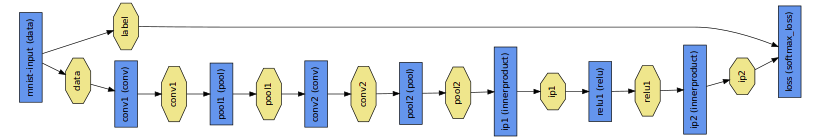
\includegraphics[width=1\textwidth]{images/caffe}}
%	\caption{An MNIST digit classification example of a Caffe network, where blue boxes represent layers and yellow octagons represent data blobs produced by or fed into the layers\cite{jia2014caffe}.}
%	\label{fig:digitnet}
%\end{figure}
\textbf{A SHORT TRANSITIVE PARAGRAPH TO GO TO RESULTS}

\subsection{Results}

In addition to the Euclidean loss function we implemented in our architecture, we use two other error measurements to evaluate and compare the performance of our model. These measurements are briefly described and justified in below:
\begin{enumerate}
\item \textbf{Mean squared error(MSE)}: Mean squared error is arguably the most important criterion used to evaluate the performance of a predictor or an estimator. The mean squared error is also useful to relay the concepts of bias, precision, and accuracy in statistical estimation. The MSE is the second moment (about the origin) of the error, and thus incorporates both the variance of the estimator and its bias \cite{lehmann1998theory}. The MSE can be estimated by
$$MSE = {\frac{1} {N}{\sum\limits_{i = 1}^N {(\hat{x_{pred}} - x_{obs} } })^{2} } $$
where:\\
\textit{N}: the number of instances\\
\textit{ $\hat{x_{pred}}$}: a vector of N predictions\\
\textit{$x_{obs}$}: a vector of observed value (ground truth) for input x\\

The mathematical benefits of mean squared error are particularly evident in its use at analyzing the performance of linear regression, as it allows one to partition the variation in a dataset into variation explained by the model and variation explained by randomness.
\item \textbf{Mean absolute error(MAE)}: MAE measures the average magnitude of the errors in a set of predictions, without considering their direction. In other words, it measures how close predictions are to the eventual outcomes \cite{willmott2005advantages}. MAE can simply be computed by:
$$MAE = {\frac{1} {N}{\sum\limits_{i = 1}^N {|x_{pred} - x_{obs} } }| } $$
where:\\
\textit{N}: number of instances\\
\textit{ $x_{pred}$}: prediction for instance x\\
\textit{$x_{obs}$}: observed value (ground truth) for instance x
\end{enumerate}

\noindent Having our used error measurements explained, for the task of counting even digits, using 800,000 training samples and 200,000 test images, and after 1,600,000 iterations, our model obtained the following results:


\begin{table}[H]
\caption{Table caption font is different from the normal text font in order to get a better differentiation -- I like it that way.}
\centering
\small\sffamily
\begin{tabular}{llr}
%\toprule
\multicolumn{2}{c}{\textbf{\textbf{Results}}} \\
\bottomrule
\textbf{Error measurement}        & \textbf{Error} \\
\bottomrule
%\midrule
Euclidean loss           & 0.20  \\
Mean squared error       & 0.20  \\
Mean absolute error      & 0.20  \\
\bottomrule
\end{tabular}
\end{table} 

Accordingly, the spread-error plot corresponding to the model is provided.

\begin{figure}[H]
	\centering
	{
\includegraphics[width=0.7\textwidth]{images/1}}
	\caption{}
	\label{fig:splot}
\end{figure}

As you may observe in Figure~\ref{fig:splot}, most
of the frames are correctly labeled. Moreover, most of the
errors correspond to adjacent number values.

A similar experiment was done by \citeauthor*{segui2015learning}. In their work, they used images with up to 5 digits with slightly different architecture. Also each digit in the images had a dimension of $28\times28$. They approached the problem as a classification task. 

\indent Therefore, in order to provide a fair comparison, we demonstrate the difference the accuracy of both experiments from random, and from there we draw a proportional comparison. These comparison has been shown in the table~\ref{tab:comp}.

\begin{table}[H]
\caption{Table caption font is different from the normal text font in order to get a better differentiation -- I like it that way.}
\centering
\small\sffamily
\begin{tabular}{llr}
%\toprule
\multicolumn{3}{c}{\textbf{\textbf{Performance Comparison}}} \\
\bottomrule
\textbf{Experiments}  & \textbf{Chance} & \textbf{Accuracy} \\
\bottomrule
%\midrule
Euclidean loss           & 0.20 & 0.30 \\
Mean squared error       & 0.20 & 0.30 \\

\bottomrule
\end{tabular}
\end{table} 

\textbf{EXPLANATION OF THE COMPARISON}

\subsection{Conclusion}

\textbf{CONCLUSION AFTER THE EXPERIMENT} 

\section{Counting pedestrians in a walkway}



\newpage

\chapter{Conclusions and Future Work}
\label{sec:conclusions}

\noindent

In this thesis we have made various contributions to the object segmentation method Cage Active Contours (CAC) originally introduced in \cite{ipcac2015}. Our contributions include 1) the introduction of two different energy functions on different color spaces which have greatly enhanced the potential of an otherwise limited method. 2) the experimental validation of our improvements with the previous energies in CAC as well as with three different related methods.  3) the formalization, in mathematical terms, of some the implications and uses of the resulting segmentation \textit{cage} (a component of CAC which is used to parametrize the contour). 4)  a highlight of the possible applications of this cage to image morphing, warping as well as in shape description. 5) the creation of a public implementation in Python (with some wrapped functions in C) of cage active contours.

\section{Conclusions}

 One of the main contributions in this work is the creation of two different energy functions. These are enhanced versions of simpler energies proposed so far in CAC which have also been extended to two different color spaces. The first one is the Multivariate Mixture Gaussian energy which is an extension to the RGB color space of the Gaussian energy defined in \cite{ipcac2015} with two more improvements: the ability to capture multiple value components in each region by using Mixture Gaussian density function, and the incorporation of an initial seed which will provide the energy with prior information about the foreground and background's distributions.

The second energy is the Mean Hue Energy, which is the analogous of the Mean Energy in \cite{ipcac2015} but on the Hue component of the HSI/HSV color spaces. Because of the Cyclic nature of the Hue component, we have had to turn to cyclic spaces to use concepts such as distance, directed distance as well as a way of finding the gradient of a of the image with respect to a control point's value.

Through quantitative and qualitative experimentation on three different datasets (section \ref{sec:experiments}), we have observed that the contribution with the most impact are the extension of the Gaussian energy to the RGB color space followed by the ability of Mixture Gaussian energies to describe a region with more than one component thus obtaining a more sophisticated representation of a region, as opposed to the polarization of pixel values in previous energies. We have also seen how the incorporation of a seed in each region does not only simplify the process but it also increases its computational speed. In the case of color images, we have seen how the Mean Hue energy, despite its simplicity, can occasionally outperform the Multivariate Mixture Gaussian energy thanks to its focus on the Hue component of the image, which reflects an intrinsic property of objects, invariant to illumination.

Furthermore, we have mathematically formalized the concepts of \textit{cage}, \textit{contour}, \textit{family of contours} and others to be able to prove that two contours are similar if their cages are similar given some intial conditions. This theoretical proof, along with the properties of mean value coordinates, used widely in computer graphic applications, have allowed us to define the conditions which allow for automatic morphing and warping between similar objects, as well provide some initial intuitions for the possibility of shape description.

Our last contribution is a public implementation of Cage Active Contours in Python with some wrappers in C. The code contains different Energy functions we have presented including the ones presented  in~\cite{ipcac2015}, as well as some tools for automatic morphing and warping. The code can be found in \url{https://github.com/Jeronics/cac-segmenter/}.


\section{Future Work}
In this work, we have also observed and pointed out the limitations that hinder the performance of the segmentation using Cage Active Contours. We have seen that CAC are not designed for high precision segmentation of arbitrary images, but rather, they provide a smooth general contour of the image which can be used for other purposes and applications. The limitations of this method can be divided into two categories: those that are dependent on energy functions and those that are dependent on the cage. 

With these considerations in mind, we have proposed a set of solutions which could be evaluated and considered for future work.

The first point to address is the cage. We have seen that the restrictions of the first stage on the vertex movements are too strong and prevent CAC from adopting complex figures. Also, they prevent the cage from rotate to better adapt to a shape. Possible solution include the weighted mean between the real direction and the projected direction or  the exploration of other internal energies that could be applied to the cage for stability.

In terms of energy functions, the most challenging task ahead, by far, is to improve the Mean Hue energy which, despite its theoretically good properties in illumination invariance, has performed poorly on the quantitative experiments on real images. However we are confident that through some improvements we could be able to rise its performance to a competent level. The first improvement we propose is the adaptation of the Gaussian Energy to this space and ultimately to the Mixture Gaussian model. This extension requires the use of analogous density functions in the cyclic domain which are known as Wrapped Density Functions. The second improvement would come from the extension of an energy to the whole HSI or HSV space. As we have concluded in section \ref{subsec:extending_to_hsi} this requires tools from directional statistics and in particular, the study of cylinder spaces which these color spaces define.

As far as the implementation goes, it would be interesting to allow for a more intuitive and user-friendly interactive interface. Some of the features this could include:
\begin{enumerate}
	\item User interaction with the cage so that control points would be able to be dragged to provide a better initialization, and to correct a segmentation at a certain point.
	\item A Morphing and Warping interface that would allow for fine-tuning of morphed objects or reassigning of correspondence in points as we have done in the morphing between the pear and apple in figure~\ref{fig:car_fruits}.
\end{enumerate} 

An interesting point we have begun to raise in this thesis is the formalization in mathematical terms of the different components in Cage Active Contours to study their properties and limitations in different applications once a segmentation has been achieved. In the process of bringing solutions, more questions are brought forward to discuss and tackle in future work. Namely: \\
Given a regular cage-configuration condition:
\begin{itemize}
	\item What is the complexity of contours that can be expressed in a contour Family?
	\item Which characteristics must a cage fulfill in order to avoid its corresponding contour to self intersect?
	\item Is there a bijective map between the equivalence classes of cages and the equivalence classes of contours in a contour Family?
\end{itemize}




\vfill
\renewcommand{\bibname}{\refname} % To change the heading of the chapter from Bibliography to References
\addcontentsline{toc}{chapter}{\bibname}

\bibliographystyle{apalike}

\bibliography{example}

%\section*{\uppercase{Appendix}}
%
%\noindent If any, the appendix should appear directly after the
%references without numbering, and not on a new page. To do so please use the following command:
%\textit{$\backslash$section*\{APPENDIX\}}
%\printglossaries %[type=\acronymtype]
\printglossary[type=\acronymtype]
\vfill
\end{document}